\documentclass[twoside]{book}

% Packages required by doxygen
\usepackage{calc}
\usepackage{doxygen}
\usepackage{graphicx}
\usepackage[utf8]{inputenc}
\usepackage{makeidx}
\usepackage{multicol}
\usepackage{multirow}
\usepackage{textcomp}
\usepackage[table]{xcolor}

% Font selection
\usepackage[T1]{fontenc}
\usepackage{mathptmx}
\usepackage[scaled=.90]{helvet}
\usepackage{courier}
\usepackage{amssymb}
\usepackage{sectsty}
\renewcommand{\familydefault}{\sfdefault}
\allsectionsfont{%
  \fontseries{bc}\selectfont%
  \color{darkgray}%
}
\renewcommand{\DoxyLabelFont}{%
  \fontseries{bc}\selectfont%
  \color{darkgray}%
}

% Page & text layout
\usepackage{geometry}
\geometry{%
  a4paper,%
  top=2.5cm,%
  bottom=2.5cm,%
  left=2.5cm,%
  right=2.5cm%
}
\tolerance=750
\hfuzz=15pt
\hbadness=750
\setlength{\emergencystretch}{15pt}
\setlength{\parindent}{0cm}
\setlength{\parskip}{0.2cm}
\makeatletter
\renewcommand{\paragraph}{%
  \@startsection{paragraph}{4}{0ex}{-1.0ex}{1.0ex}{%
    \normalfont\normalsize\bfseries\SS@parafont%
  }%
}
\renewcommand{\subparagraph}{%
  \@startsection{subparagraph}{5}{0ex}{-1.0ex}{1.0ex}{%
    \normalfont\normalsize\bfseries\SS@subparafont%
  }%
}
\makeatother

% Headers & footers
\usepackage{fancyhdr}
\pagestyle{fancyplain}
\fancyhead[LE]{\fancyplain{}{\bfseries\thepage}}
\fancyhead[CE]{\fancyplain{}{}}
\fancyhead[RE]{\fancyplain{}{\bfseries\leftmark}}
\fancyhead[LO]{\fancyplain{}{\bfseries\rightmark}}
\fancyhead[CO]{\fancyplain{}{}}
\fancyhead[RO]{\fancyplain{}{\bfseries\thepage}}
\fancyfoot[LE]{\fancyplain{}{}}
\fancyfoot[CE]{\fancyplain{}{}}
\fancyfoot[RE]{\fancyplain{}{\bfseries\scriptsize Generated on Tue Jun 25 2013 09:58:12 for Canary API by Doxygen }}
\fancyfoot[LO]{\fancyplain{}{\bfseries\scriptsize Generated on Tue Jun 25 2013 09:58:12 for Canary API by Doxygen }}
\fancyfoot[CO]{\fancyplain{}{}}
\fancyfoot[RO]{\fancyplain{}{}}
\renewcommand{\footrulewidth}{0.4pt}
\renewcommand{\chaptermark}[1]{%
  \markboth{#1}{}%
}
\renewcommand{\sectionmark}[1]{%
  \markright{\thesection\ #1}%
}

% Indices & bibliography
\usepackage{natbib}
\usepackage[titles]{tocloft}
\setcounter{tocdepth}{3}
\setcounter{secnumdepth}{5}
\makeindex

% Hyperlinks (required, but should be loaded last)
\usepackage{ifpdf}
\ifpdf
  \usepackage[pdftex,pagebackref=true]{hyperref}
\else
  \usepackage[ps2pdf,pagebackref=true]{hyperref}
\fi
\hypersetup{%
  colorlinks=true,%
  linkcolor=blue,%
  citecolor=blue,%
  unicode%
}

% Custom commands
\newcommand{\clearemptydoublepage}{%
  \newpage{\pagestyle{empty}\cleardoublepage}%
}


%===== C O N T E N T S =====

\begin{document}

% Titlepage & ToC
\hypersetup{pageanchor=false}
\pagenumbering{roman}
\begin{titlepage}
\vspace*{7cm}
\begin{center}%
{\Large Canary A\-P\-I \\[1ex]\large 1.\-0 }\\
\vspace*{1cm}
{\large Generated by Doxygen 1.8.4}\\
\vspace*{0.5cm}
{\small Tue Jun 25 2013 09:58:12}\\
\end{center}
\end{titlepage}
\clearemptydoublepage
\tableofcontents
\clearemptydoublepage
\pagenumbering{arabic}
\hypersetup{pageanchor=true}

%--- Begin generated contents ---
\chapter{Canary\-A\-P\-I}
\label{md_README}
\hypertarget{md_README}{}
Dependencies\-:

Tornado Tornadio2 \-: \href{https://github.com/mrjoes/tornadio2}{\tt https\-://github.\-com/mrjoes/tornadio2} 
\chapter{Namespace Index}
\section{Namespace List}
Here is a list of all documented namespaces with brief descriptions\-:\begin{DoxyCompactList}
\item\contentsline{section}{\hyperlink{namespaceapi}{api} }{\pageref{namespaceapi}}{}
\item\contentsline{section}{\hyperlink{namespace_canary_assets_1_1_device}{Canary\-Assets.\-Device} }{\pageref{namespace_canary_assets_1_1_device}}{}
\item\contentsline{section}{\hyperlink{namespace_canary_assets_1_1_nest}{Canary\-Assets.\-Nest} }{\pageref{namespace_canary_assets_1_1_nest}}{}
\item\contentsline{section}{\hyperlink{namespace_canary_assets_1_1_user}{Canary\-Assets.\-User} }{\pageref{namespace_canary_assets_1_1_user}}{}
\item\contentsline{section}{\hyperlink{namespace_canary_models_1_1_battery}{Canary\-Models.\-Battery} }{\pageref{namespace_canary_models_1_1_battery}}{}
\item\contentsline{section}{\hyperlink{namespace_canary_models_1_1_c_o}{Canary\-Models.\-C\-O} }{\pageref{namespace_canary_models_1_1_c_o}}{}
\item\contentsline{section}{\hyperlink{namespace_canary_models_1_1_c_o2}{Canary\-Models.\-C\-O2} }{\pageref{namespace_canary_models_1_1_c_o2}}{}
\item\contentsline{section}{\hyperlink{namespace_canary_models_1_1_nearby_hazard}{Canary\-Models.\-Nearby\-Hazard} }{\pageref{namespace_canary_models_1_1_nearby_hazard}}{}
\item\contentsline{section}{\hyperlink{namespace_canary_models_1_1_n_o2}{Canary\-Models.\-N\-O2} }{\pageref{namespace_canary_models_1_1_n_o2}}{}
\item\contentsline{section}{\hyperlink{namespace_canary_models_1_1_outdoor_quality}{Canary\-Models.\-Outdoor\-Quality} }{\pageref{namespace_canary_models_1_1_outdoor_quality}}{}
\item\contentsline{section}{\hyperlink{namespace_canary_models_1_1_p_m10}{Canary\-Models.\-P\-M10} }{\pageref{namespace_canary_models_1_1_p_m10}}{}
\item\contentsline{section}{\hyperlink{namespace_canary_models_1_1_p_m2__5}{Canary\-Models.\-P\-M2\-\_\-5} }{\pageref{namespace_canary_models_1_1_p_m2__5}}{}
\item\contentsline{section}{\hyperlink{namespace_canary_models_1_1_smoke}{Canary\-Models.\-Smoke} }{\pageref{namespace_canary_models_1_1_smoke}}{}
\item\contentsline{section}{\hyperlink{namespace_canary_models_1_1_temperature}{Canary\-Models.\-Temperature} }{\pageref{namespace_canary_models_1_1_temperature}}{}
\item\contentsline{section}{\hyperlink{namespace_canary_utils_1_1_authentication}{Canary\-Utils.\-Authentication} }{\pageref{namespace_canary_utils_1_1_authentication}}{}
\end{DoxyCompactList}

\chapter{Hierarchical Index}
\section{Class Hierarchy}
This inheritance list is sorted roughly, but not completely, alphabetically\-:\begin{DoxyCompactList}
\item \contentsline{section}{Canary\-Assets.\-Asset.\-Asset}{\pageref{class_canary_assets_1_1_asset_1_1_asset}}{}
\item \contentsline{section}{api.\-Canary\-Call}{\pageref{classapi_1_1_canary_call}}{}
\item \contentsline{section}{Canary\-Models.\-Model.\-Model}{\pageref{class_canary_models_1_1_model_1_1_model}}{}
\item Request\-Handler\begin{DoxyCompactList}
\item \contentsline{section}{api.\-Communicator}{\pageref{classapi_1_1_communicator}}{}
\item \contentsline{section}{api.\-Device}{\pageref{classapi_1_1_device}}{}
\item \contentsline{section}{api.\-Devices}{\pageref{classapi_1_1_devices}}{}
\item \contentsline{section}{api.\-Nest}{\pageref{classapi_1_1_nest}}{}
\item \contentsline{section}{api.\-Nests}{\pageref{classapi_1_1_nests}}{}
\item \contentsline{section}{api.\-Ping}{\pageref{classapi_1_1_ping}}{}
\item \contentsline{section}{api.\-User}{\pageref{classapi_1_1_user}}{}
\item \contentsline{section}{api.\-Users}{\pageref{classapi_1_1_users}}{}
\item \contentsline{section}{hailingfrequency.\-Hailing\-Frequency\-Handler}{\pageref{classhailingfrequency_1_1_hailing_frequency_handler}}{}
\item \contentsline{section}{hailingfrequency.\-Socket\-I\-O\-Handler}{\pageref{classhailingfrequency_1_1_socket_i_o_handler}}{}
\end{DoxyCompactList}
\item Socket\-Connection\begin{DoxyCompactList}
\item \contentsline{section}{hailingfrequency.\-Hailing\-Frequency}{\pageref{classhailingfrequency_1_1_hailing_frequency}}{}
\item \contentsline{section}{hailingfrequency.\-Router}{\pageref{classhailingfrequency_1_1_router}}{}
\end{DoxyCompactList}
\item Asset\begin{DoxyCompactList}
\item \contentsline{section}{Canary\-Assets.\-Device.\-Device}{\pageref{class_canary_assets_1_1_device_1_1_device}}{}
\item \contentsline{section}{Canary\-Assets.\-Nest.\-Nest}{\pageref{class_canary_assets_1_1_nest_1_1_nest}}{}
\item \contentsline{section}{Canary\-Assets.\-User.\-User}{\pageref{class_canary_assets_1_1_user_1_1_user}}{}
\end{DoxyCompactList}
\item Model\begin{DoxyCompactList}
\item \contentsline{section}{Canary\-Models.\-Battery.\-Battery}{\pageref{class_canary_models_1_1_battery_1_1_battery}}{}
\item \contentsline{section}{Canary\-Models.\-C\-O2.\-C\-O2}{\pageref{class_canary_models_1_1_c_o2_1_1_c_o2}}{}
\item \contentsline{section}{Canary\-Models.\-C\-O.\-C\-O}{\pageref{class_canary_models_1_1_c_o_1_1_c_o}}{}
\item \contentsline{section}{Canary\-Models.\-Nearby\-Hazard.\-Nearby\-Hazard}{\pageref{class_canary_models_1_1_nearby_hazard_1_1_nearby_hazard}}{}
\item \contentsline{section}{Canary\-Models.\-N\-O2.\-N\-O2}{\pageref{class_canary_models_1_1_n_o2_1_1_n_o2}}{}
\item \contentsline{section}{Canary\-Models.\-Outdoor\-Quality.\-Outdoor\-Quality}{\pageref{class_canary_models_1_1_outdoor_quality_1_1_outdoor_quality}}{}
\item \contentsline{section}{Canary\-Models.\-P\-M10.\-P\-M10}{\pageref{class_canary_models_1_1_p_m10_1_1_p_m10}}{}
\item \contentsline{section}{Canary\-Models.\-P\-M2\-\_\-5.\-P\-M2\-\_\-5}{\pageref{class_canary_models_1_1_p_m2__5_1_1_p_m2__5}}{}
\item \contentsline{section}{Canary\-Models.\-Smoke.\-Smoke}{\pageref{class_canary_models_1_1_smoke_1_1_smoke}}{}
\item \contentsline{section}{Canary\-Models.\-Temperature.\-Temperature}{\pageref{class_canary_models_1_1_temperature_1_1_temperature}}{}
\end{DoxyCompactList}
\end{DoxyCompactList}

\chapter{Class Index}
\section{Class List}
Here are the classes, structs, unions and interfaces with brief descriptions\-:\begin{DoxyCompactList}
\item\contentsline{section}{\hyperlink{classasset_1_1_asset}{asset.\-Asset} }{\pageref{classasset_1_1_asset}}{}
\item\contentsline{section}{\hyperlink{classapi_1_1_canary_call}{api.\-Canary\-Call} }{\pageref{classapi_1_1_canary_call}}{}
\item\contentsline{section}{\hyperlink{classapi_1_1_communicator}{api.\-Communicator} }{\pageref{classapi_1_1_communicator}}{}
\item\contentsline{section}{\hyperlink{classdevice_1_1_device}{device.\-Device} }{\pageref{classdevice_1_1_device}}{}
\item\contentsline{section}{\hyperlink{classapi_1_1_device}{api.\-Device} }{\pageref{classapi_1_1_device}}{}
\item\contentsline{section}{\hyperlink{classapi_1_1_devices}{api.\-Devices} }{\pageref{classapi_1_1_devices}}{}
\item\contentsline{section}{\hyperlink{classhailingfrequency_1_1_hailing_frequency}{hailingfrequency.\-Hailing\-Frequency} }{\pageref{classhailingfrequency_1_1_hailing_frequency}}{}
\item\contentsline{section}{\hyperlink{classhailingfrequency_1_1_hailing_frequency_handler}{hailingfrequency.\-Hailing\-Frequency\-Handler} }{\pageref{classhailingfrequency_1_1_hailing_frequency_handler}}{}
\item\contentsline{section}{\hyperlink{classapi_1_1_nest}{api.\-Nest} }{\pageref{classapi_1_1_nest}}{}
\item\contentsline{section}{\hyperlink{classnest_1_1_nest}{nest.\-Nest} }{\pageref{classnest_1_1_nest}}{}
\item\contentsline{section}{\hyperlink{classapi_1_1_nests}{api.\-Nests} }{\pageref{classapi_1_1_nests}}{}
\item\contentsline{section}{\hyperlink{classapi_1_1_ping}{api.\-Ping} }{\pageref{classapi_1_1_ping}}{}
\item\contentsline{section}{\hyperlink{classhailingfrequency_1_1_router}{hailingfrequency.\-Router} }{\pageref{classhailingfrequency_1_1_router}}{}
\item\contentsline{section}{\hyperlink{classhailingfrequency_1_1_socket_i_o_handler}{hailingfrequency.\-Socket\-I\-O\-Handler} }{\pageref{classhailingfrequency_1_1_socket_i_o_handler}}{}
\item\contentsline{section}{\hyperlink{classuser_1_1_user}{user.\-User} }{\pageref{classuser_1_1_user}}{}
\item\contentsline{section}{\hyperlink{classapi_1_1_user}{api.\-User} }{\pageref{classapi_1_1_user}}{}
\item\contentsline{section}{\hyperlink{classapi_1_1_users}{api.\-Users} }{\pageref{classapi_1_1_users}}{}
\end{DoxyCompactList}

\chapter{Namespace Documentation}
\hypertarget{namespaceapi}{\section{api Namespace Reference}
\label{namespaceapi}\index{api@{api}}
}
\subsection*{Classes}
\begin{DoxyCompactItemize}
\item 
class \hyperlink{classapi_1_1_canary_call}{Canary\-Call}
\item 
class \hyperlink{classapi_1_1_users}{Users}
\item 
class \hyperlink{classapi_1_1_user}{User}
\item 
class \hyperlink{classapi_1_1_nests}{Nests}
\item 
class \hyperlink{classapi_1_1_nest}{Nest}
\item 
class \hyperlink{classapi_1_1_devices}{Devices}
\item 
class \hyperlink{classapi_1_1_device}{Device}
\item 
class \hyperlink{classapi_1_1_ping}{Ping}
\item 
class \hyperlink{classapi_1_1_status}{Status}
\item 
class \hyperlink{classapi_1_1_communicator}{Communicator}
\end{DoxyCompactItemize}
\subsection*{Variables}
\begin{DoxyCompactItemize}
\item 
tuple {\bfseries api}
\item 
\hypertarget{namespaceapi_a1125afafaabf4d39e0f633946f62eecd}{tuple {\bfseries http\-\_\-server} = tornado.\-httpserver.\-H\-T\-T\-P\-Server(api)}\label{namespaceapi_a1125afafaabf4d39e0f633946f62eecd}

\end{DoxyCompactItemize}


\subsection{Detailed Description}
\begin{DoxyVerb}@package Canary.Api

The main API for the cloud-based service.
\end{DoxyVerb}
 

\subsection{Variable Documentation}
\hypertarget{namespaceapi_a5697ea202319f894facccacf78d93e89}{\index{api@{api}!api@{api}}
\index{api@{api}!api@{api}}
\subsubsection[{api}]{\setlength{\rightskip}{0pt plus 5cm}tuple api.\-api}}\label{namespaceapi_a5697ea202319f894facccacf78d93e89}
{\bfseries Initial value\-:}
\begin{DoxyCode}
1 = tornado.web.Application([
2     (\textcolor{stringliteral}{r"/users/"}, Users),
3     (\textcolor{stringliteral}{r"/user/(.*)/"}, User, dict(userId = \textcolor{keywordtype}{None})),
4     (\textcolor{stringliteral}{r"/nests/"}, Nests),
5     (\textcolor{stringliteral}{r"/nest/(.*)/"}, Nest, dict(nestId = \textcolor{keywordtype}{None})),
6     (\textcolor{stringliteral}{r"/nest/(.*)/communicator/"}, Communicator, dict(nestId = \textcolor{keywordtype}{None})),
7     (\textcolor{stringliteral}{r"/devices/"}, Devices),
8     (\textcolor{stringliteral}{r"/device/(.*)/"}, Device, dict(deviceId = \textcolor{keywordtype}{None})),
9     (\textcolor{stringliteral}{r"/ping/(.*)/(.*)/"}, Ping, dict(entityId = \textcolor{keywordtype}{None}, action = \textcolor{keywordtype}{None})),
10     (\textcolor{stringliteral}{r"/status/(.*)/(.*)/"}, Status, dict(entityId = \textcolor{keywordtype}{None}, status = \textcolor{keywordtype}{None})),
11     
12     (\textcolor{stringliteral}{r"/docs/(.*)"}, tornado.web.StaticFileHandler, \{\textcolor{stringliteral}{'path'}: globals.docs\_path\}),    \textcolor{comment}{# helpers; remove in
       production}
13     (\textcolor{stringliteral}{r"/communicator/"}, HailingFrequencyHandler),
14     (\textcolor{stringliteral}{r"/js/socket.io.js"}, SocketIOHandler)
15 ])
\end{DoxyCode}

\hypertarget{namespaceasset}{\section{asset Namespace Reference}
\label{namespaceasset}\index{asset@{asset}}
}
\subsection*{Classes}
\begin{DoxyCompactItemize}
\item 
class \hyperlink{classasset_1_1_asset}{Asset}
\end{DoxyCompactItemize}
\subsection*{Variables}
\begin{DoxyCompactItemize}
\item 
\hypertarget{namespaceasset_a2ae80da3053a8479180d469002bf93cf}{{\bfseries \-\_\-\-\_\-metaclass\-\_\-\-\_\-} = type}\label{namespaceasset_a2ae80da3053a8479180d469002bf93cf}

\end{DoxyCompactItemize}


\subsection{Detailed Description}
\begin{DoxyVerb}@package Canary.Asset

This is a test!
\end{DoxyVerb}
 
\hypertarget{namespacedevice}{\section{device Namespace Reference}
\label{namespacedevice}\index{device@{device}}
}
\subsection*{Classes}
\begin{DoxyCompactItemize}
\item 
class \hyperlink{classdevice_1_1_device}{Device}
\end{DoxyCompactItemize}
\subsection*{Variables}
\begin{DoxyCompactItemize}
\item 
dictionary {\bfseries status}
\end{DoxyCompactItemize}


\subsection{Detailed Description}
\begin{DoxyVerb}@package Canary.Asset.Device

Device is a subclass of Asset
\end{DoxyVerb}
 

\subsection{Variable Documentation}
\hypertarget{namespacedevice_a9d055d66be48177d3fa562943d9ffc9e}{\index{device@{device}!status@{status}}
\index{status@{status}!device@{device}}
\subsubsection[{status}]{\setlength{\rightskip}{0pt plus 5cm}dictionary device.\-status}}\label{namespacedevice_a9d055d66be48177d3fa562943d9ffc9e}
{\bfseries Initial value\-:}
\begin{DoxyCode}
1 = \{
2     \textcolor{stringliteral}{'battery'}: 0.0,
3     \textcolor{stringliteral}{'monoxide'}: 0.0,
4     \textcolor{stringliteral}{'air\_quality'}: 0.0  
5 \}
\end{DoxyCode}

\hypertarget{namespacenest}{\section{nest Namespace Reference}
\label{namespacenest}\index{nest@{nest}}
}
\subsection*{Classes}
\begin{DoxyCompactItemize}
\item 
class \hyperlink{classnest_1_1_nest}{Nest}
\end{DoxyCompactItemize}
\subsection*{Variables}
\begin{DoxyCompactItemize}
\item 
\hypertarget{namespacenest_a5dd443347ff8776c0e1c6d2ba4225845}{list {\bfseries members} = \mbox{[}$\,$\mbox{]}}\label{namespacenest_a5dd443347ff8776c0e1c6d2ba4225845}

\item 
\hypertarget{namespacenest_ab730b69fd5eac5a436265a501613b55c}{list {\bfseries devices} = \mbox{[}$\,$\mbox{]}}\label{namespacenest_ab730b69fd5eac5a436265a501613b55c}

\end{DoxyCompactItemize}


\subsection{Detailed Description}
\begin{DoxyVerb}@package Canary.Asset.Nest

Nest is a subclass of Asset
\end{DoxyVerb}
 
\hypertarget{namespaceuser}{\section{user Namespace Reference}
\label{namespaceuser}\index{user@{user}}
}
\subsection*{Classes}
\begin{DoxyCompactItemize}
\item 
class \hyperlink{classuser_1_1_user}{User}
\end{DoxyCompactItemize}
\subsection*{Variables}
\begin{DoxyCompactItemize}
\item 
\hypertarget{namespaceuser_a6da2acf5ac2587e104d2f8adaa99177d}{list {\bfseries nests} = \mbox{[}$\,$\mbox{]}}\label{namespaceuser_a6da2acf5ac2587e104d2f8adaa99177d}

\end{DoxyCompactItemize}


\subsection{Detailed Description}
\begin{DoxyVerb}@package Canary.Asset.User

User is a subclass of Asset
\end{DoxyVerb}
 
\chapter{Class Documentation}
\hypertarget{classasset_1_1_asset}{\section{asset.\-Asset Class Reference}
\label{classasset_1_1_asset}\index{asset.\-Asset@{asset.\-Asset}}
}
Inheritance diagram for asset.\-Asset\-:\begin{figure}[H]
\begin{center}
\leavevmode
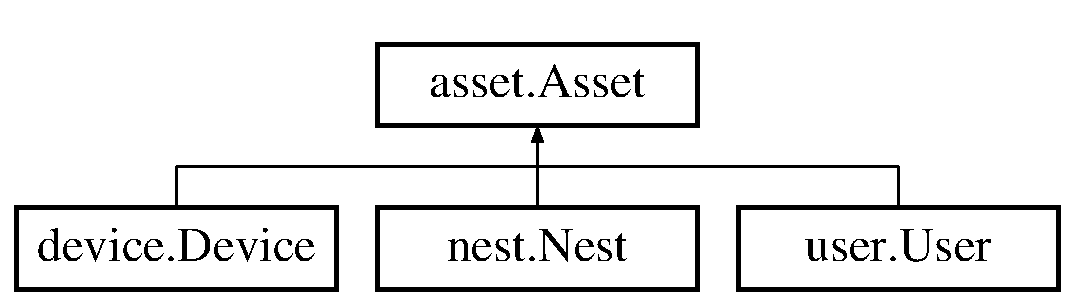
\includegraphics[height=2.000000cm]{classasset_1_1_asset}
\end{center}
\end{figure}
\subsection*{Public Member Functions}
\begin{DoxyCompactItemize}
\item 
\hypertarget{classasset_1_1_asset_a1d5701776cb8a710192c9b1d356e76bc}{def {\bfseries \-\_\-\-\_\-init\-\_\-\-\_\-}}\label{classasset_1_1_asset_a1d5701776cb8a710192c9b1d356e76bc}

\item 
def \hyperlink{classasset_1_1_asset_a7628151c7b06d24d0150107681e90f59}{create}
\item 
\hypertarget{classasset_1_1_asset_aa64bdb5546de358c271232f0fb4863f8}{def {\bfseries emit}}\label{classasset_1_1_asset_aa64bdb5546de358c271232f0fb4863f8}

\end{DoxyCompactItemize}
\subsection*{Static Public Attributes}
\begin{DoxyCompactItemize}
\item 
\hypertarget{classasset_1_1_asset_ad539bb2223a6c5f80d432f07ff2742cf}{{\bfseries entity\-Id} = None}\label{classasset_1_1_asset_ad539bb2223a6c5f80d432f07ff2742cf}

\item 
\hypertarget{classasset_1_1_asset_a0cbfe18462e6929345578c21ce4603d7}{list {\bfseries accepted\-Keys} = \mbox{[}$\,$\mbox{]}}\label{classasset_1_1_asset_a0cbfe18462e6929345578c21ce4603d7}

\end{DoxyCompactItemize}


\subsection{Detailed Description}
\begin{DoxyVerb}The Asset superclass encapsulates all entities (Users, Nests, Devices).  Its acceptedKeys indicates which users may have access to its methods.\end{DoxyVerb}
 

\subsection{Member Function Documentation}
\hypertarget{classasset_1_1_asset_a7628151c7b06d24d0150107681e90f59}{\index{asset\-::\-Asset@{asset\-::\-Asset}!create@{create}}
\index{create@{create}!asset::Asset@{asset\-::\-Asset}}
\subsubsection[{create}]{\setlength{\rightskip}{0pt plus 5cm}def asset.\-Asset.\-create (
\begin{DoxyParamCaption}
\item[{}]{self}
\end{DoxyParamCaption}
)}}\label{classasset_1_1_asset_a7628151c7b06d24d0150107681e90f59}
\begin{DoxyVerb}Creates a new Asset, and sets its id.\end{DoxyVerb}
 

The documentation for this class was generated from the following file\-:\begin{DoxyCompactItemize}
\item 
asset.\-py\end{DoxyCompactItemize}

\hypertarget{classapi_1_1_canary_call}{\section{api.\-Canary\-Call Class Reference}
\label{classapi_1_1_canary_call}\index{api.\-Canary\-Call@{api.\-Canary\-Call}}
}
\subsection*{Public Member Functions}
\begin{DoxyCompactItemize}
\item 
def \hyperlink{classapi_1_1_canary_call_ac588d521c86e5fc5c12f1b3726a64c43}{\-\_\-\-\_\-init\-\_\-\-\_\-}
\item 
def \hyperlink{classapi_1_1_canary_call_a6bfc31d394a2d0009114243d157fe2ed}{emit}
\end{DoxyCompactItemize}
\subsection*{Public Attributes}
\begin{DoxyCompactItemize}
\item 
\hypertarget{classapi_1_1_canary_call_a7e92b23fd21be88cfed022b4a6939040}{{\bfseries result}}\label{classapi_1_1_canary_call_a7e92b23fd21be88cfed022b4a6939040}

\item 
\hypertarget{classapi_1_1_canary_call_a863215d250eb3714a11462265a04c9e3}{{\bfseries data}}\label{classapi_1_1_canary_call_a863215d250eb3714a11462265a04c9e3}

\end{DoxyCompactItemize}


\subsection{Constructor \& Destructor Documentation}
\hypertarget{classapi_1_1_canary_call_ac588d521c86e5fc5c12f1b3726a64c43}{\index{api\-::\-Canary\-Call@{api\-::\-Canary\-Call}!\-\_\-\-\_\-init\-\_\-\-\_\-@{\-\_\-\-\_\-init\-\_\-\-\_\-}}
\index{\-\_\-\-\_\-init\-\_\-\-\_\-@{\-\_\-\-\_\-init\-\_\-\-\_\-}!api::CanaryCall@{api\-::\-Canary\-Call}}
\subsubsection[{\-\_\-\-\_\-init\-\_\-\-\_\-}]{\setlength{\rightskip}{0pt plus 5cm}def api.\-Canary\-Call.\-\_\-\-\_\-init\-\_\-\-\_\- (
\begin{DoxyParamCaption}
\item[{}]{self, }
\item[{}]{result = {\ttfamily None}}
\end{DoxyParamCaption}
)}}\label{classapi_1_1_canary_call_ac588d521c86e5fc5c12f1b3726a64c43}
\begin{DoxyVerb}You may pass CanaryCall an object to set as its data (i.e. the result of a query).  If data is present, the result will automatically be set to 200 (OK).\end{DoxyVerb}
 

\subsection{Member Function Documentation}
\hypertarget{classapi_1_1_canary_call_a6bfc31d394a2d0009114243d157fe2ed}{\index{api\-::\-Canary\-Call@{api\-::\-Canary\-Call}!emit@{emit}}
\index{emit@{emit}!api::CanaryCall@{api\-::\-Canary\-Call}}
\subsubsection[{emit}]{\setlength{\rightskip}{0pt plus 5cm}def api.\-Canary\-Call.\-emit (
\begin{DoxyParamCaption}
\item[{}]{self}
\end{DoxyParamCaption}
)}}\label{classapi_1_1_canary_call_a6bfc31d394a2d0009114243d157fe2ed}
\begin{DoxyVerb}Returns the CanaryCall object as a dict, which can be output as JSON\end{DoxyVerb}
 

The documentation for this class was generated from the following file\-:\begin{DoxyCompactItemize}
\item 
api.\-py\end{DoxyCompactItemize}

\hypertarget{classapi_1_1_communicator}{\section{api.\-Communicator Class Reference}
\label{classapi_1_1_communicator}\index{api.\-Communicator@{api.\-Communicator}}
}
Inheritance diagram for api.\-Communicator\-:\begin{figure}[H]
\begin{center}
\leavevmode
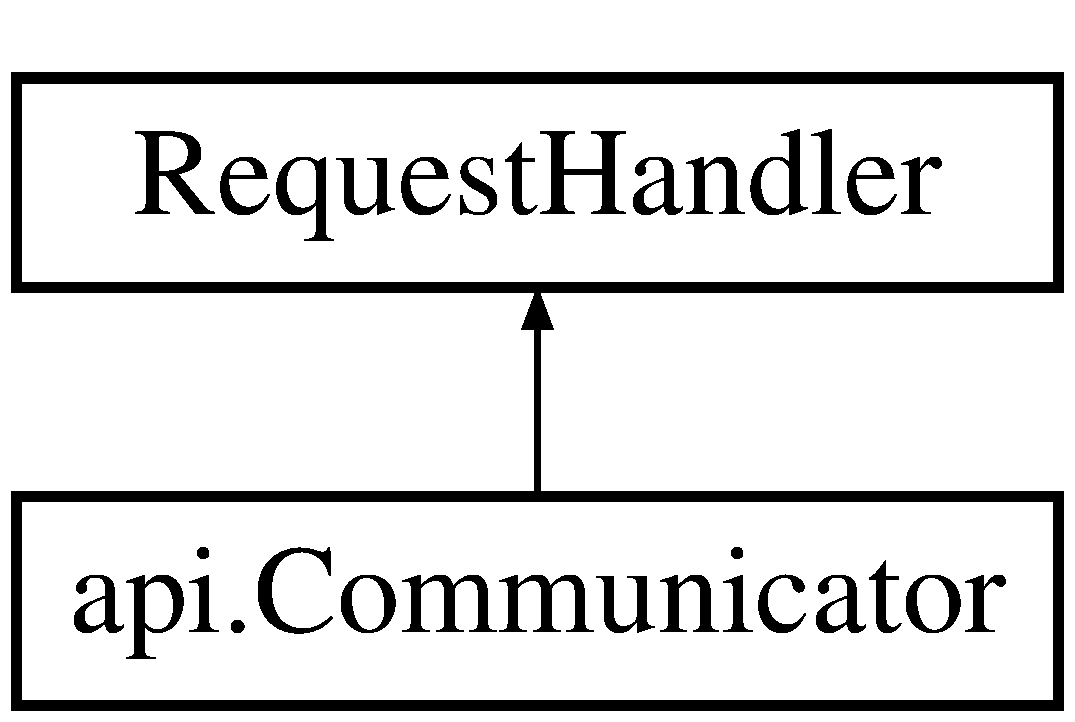
\includegraphics[height=2.000000cm]{classapi_1_1_communicator}
\end{center}
\end{figure}
\subsection*{Public Member Functions}
\begin{DoxyCompactItemize}
\item 
\hypertarget{classapi_1_1_communicator_a52ef801f9faaf4195e3824aba8ac1d65}{def {\bfseries initialize}}\label{classapi_1_1_communicator_a52ef801f9faaf4195e3824aba8ac1d65}

\item 
def \hyperlink{classapi_1_1_communicator_abc45b289619e0988116e80b35b7fabb9}{get}
\item 
def \hyperlink{classapi_1_1_communicator_acf9eee605fa05aafd4ef7b9caa7e3064}{post}
\item 
def \hyperlink{classapi_1_1_communicator_a7b1910fd8ee6416508032e9c533634da}{delete}
\item 
def \hyperlink{classapi_1_1_communicator_af5958bce2d64cec51a03c6c27b44122c}{put}
\end{DoxyCompactItemize}
\subsection*{Public Attributes}
\begin{DoxyCompactItemize}
\item 
\hypertarget{classapi_1_1_communicator_ad81c8f11473c4779f45fb7ca8993b5bd}{{\bfseries nest\-Id}}\label{classapi_1_1_communicator_ad81c8f11473c4779f45fb7ca8993b5bd}

\end{DoxyCompactItemize}


\subsection{Member Function Documentation}
\hypertarget{classapi_1_1_communicator_a7b1910fd8ee6416508032e9c533634da}{\index{api\-::\-Communicator@{api\-::\-Communicator}!delete@{delete}}
\index{delete@{delete}!api::Communicator@{api\-::\-Communicator}}
\subsubsection[{delete}]{\setlength{\rightskip}{0pt plus 5cm}def api.\-Communicator.\-delete (
\begin{DoxyParamCaption}
\item[{}]{self, }
\item[{}]{nest\-Id}
\end{DoxyParamCaption}
)}}\label{classapi_1_1_communicator_a7b1910fd8ee6416508032e9c533634da}
\begin{DoxyVerb}DELETE: ends the currently open communication session between members of a Nest.\end{DoxyVerb}
 \hypertarget{classapi_1_1_communicator_abc45b289619e0988116e80b35b7fabb9}{\index{api\-::\-Communicator@{api\-::\-Communicator}!get@{get}}
\index{get@{get}!api::Communicator@{api\-::\-Communicator}}
\subsubsection[{get}]{\setlength{\rightskip}{0pt plus 5cm}def api.\-Communicator.\-get (
\begin{DoxyParamCaption}
\item[{}]{self, }
\item[{}]{nest\-Id}
\end{DoxyParamCaption}
)}}\label{classapi_1_1_communicator_abc45b289619e0988116e80b35b7fabb9}
\begin{DoxyVerb}GET: gets the current communication session opened between members of a Nest, or null if uninitiated.\end{DoxyVerb}
 \hypertarget{classapi_1_1_communicator_acf9eee605fa05aafd4ef7b9caa7e3064}{\index{api\-::\-Communicator@{api\-::\-Communicator}!post@{post}}
\index{post@{post}!api::Communicator@{api\-::\-Communicator}}
\subsubsection[{post}]{\setlength{\rightskip}{0pt plus 5cm}def api.\-Communicator.\-post (
\begin{DoxyParamCaption}
\item[{}]{self, }
\item[{}]{nest\-Id}
\end{DoxyParamCaption}
)}}\label{classapi_1_1_communicator_acf9eee605fa05aafd4ef7b9caa7e3064}
\begin{DoxyVerb}POST: starts a new communication session between members of a Nest.\end{DoxyVerb}
 \hypertarget{classapi_1_1_communicator_af5958bce2d64cec51a03c6c27b44122c}{\index{api\-::\-Communicator@{api\-::\-Communicator}!put@{put}}
\index{put@{put}!api::Communicator@{api\-::\-Communicator}}
\subsubsection[{put}]{\setlength{\rightskip}{0pt plus 5cm}def api.\-Communicator.\-put (
\begin{DoxyParamCaption}
\item[{}]{self, }
\item[{}]{nest\-Id}
\end{DoxyParamCaption}
)}}\label{classapi_1_1_communicator_af5958bce2d64cec51a03c6c27b44122c}
\begin{DoxyVerb}PUT: updates the currently open communication session between members of a Nest.\end{DoxyVerb}
 

The documentation for this class was generated from the following file\-:\begin{DoxyCompactItemize}
\item 
api.\-py\end{DoxyCompactItemize}

\hypertarget{classdevice_1_1_device}{\section{device.\-Device Class Reference}
\label{classdevice_1_1_device}\index{device.\-Device@{device.\-Device}}
}
Inheritance diagram for device.\-Device\-:\begin{figure}[H]
\begin{center}
\leavevmode
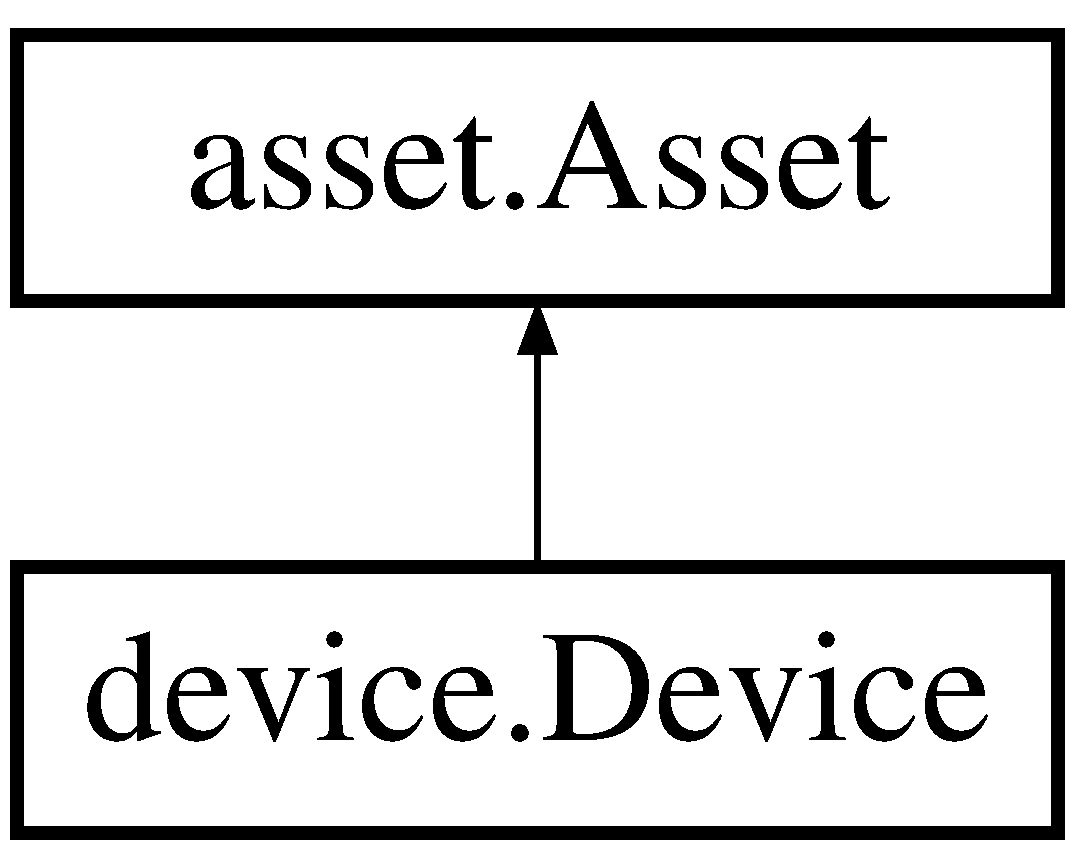
\includegraphics[height=2.000000cm]{classdevice_1_1_device}
\end{center}
\end{figure}
\subsection*{Public Member Functions}
\begin{DoxyCompactItemize}
\item 
\hypertarget{classdevice_1_1_device_a63b14186c2c1f3176f253b28015c5fd0}{def {\bfseries \-\_\-\-\_\-init\-\_\-\-\_\-}}\label{classdevice_1_1_device_a63b14186c2c1f3176f253b28015c5fd0}

\item 
def \hyperlink{classdevice_1_1_device_a16b72d4e5916569c4fdbb99bc0850f9b}{create}
\end{DoxyCompactItemize}
\subsection*{Public Attributes}
\begin{DoxyCompactItemize}
\item 
\hypertarget{classdevice_1_1_device_a4c85d31437d42a37b9b9e413261c7333}{{\bfseries status}}\label{classdevice_1_1_device_a4c85d31437d42a37b9b9e413261c7333}

\end{DoxyCompactItemize}
\subsection*{Additional Inherited Members}


\subsection{Member Function Documentation}
\hypertarget{classdevice_1_1_device_a16b72d4e5916569c4fdbb99bc0850f9b}{\index{device\-::\-Device@{device\-::\-Device}!create@{create}}
\index{create@{create}!device::Device@{device\-::\-Device}}
\subsubsection[{create}]{\setlength{\rightskip}{0pt plus 5cm}def device.\-Device.\-create (
\begin{DoxyParamCaption}
\item[{}]{self}
\end{DoxyParamCaption}
)}}\label{classdevice_1_1_device_a16b72d4e5916569c4fdbb99bc0850f9b}
\begin{DoxyVerb}Creates a new Device, and sets its id.\end{DoxyVerb}
 

The documentation for this class was generated from the following file\-:\begin{DoxyCompactItemize}
\item 
device.\-py\end{DoxyCompactItemize}

\hypertarget{classapi_1_1_device}{\section{api.\-Device Class Reference}
\label{classapi_1_1_device}\index{api.\-Device@{api.\-Device}}
}
Inheritance diagram for api.\-Device\-:\begin{figure}[H]
\begin{center}
\leavevmode
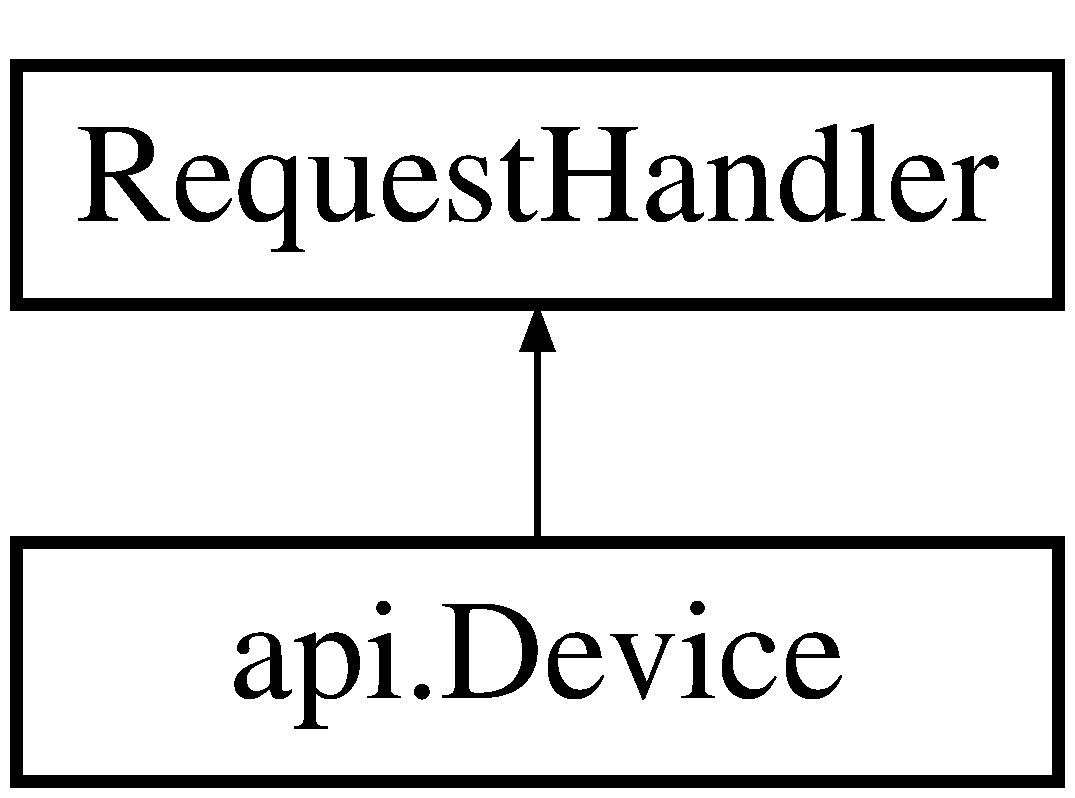
\includegraphics[height=2.000000cm]{classapi_1_1_device}
\end{center}
\end{figure}
\subsection*{Public Member Functions}
\begin{DoxyCompactItemize}
\item 
\hypertarget{classapi_1_1_device_abe43b29a0471c001944bb1634ead3165}{def {\bfseries initialize}}\label{classapi_1_1_device_abe43b29a0471c001944bb1634ead3165}

\item 
def \hyperlink{classapi_1_1_device_aab84744b823a1e3f44700c9ba50d5051}{get}
\item 
def \hyperlink{classapi_1_1_device_ae051140ce5b14440b74a6634c27ee4c0}{put}
\item 
def \hyperlink{classapi_1_1_device_aa1b4c05ad4a3331e80331754055c0ec9}{delete}
\end{DoxyCompactItemize}
\subsection*{Public Attributes}
\begin{DoxyCompactItemize}
\item 
\hypertarget{classapi_1_1_device_a0190a4c54d0998cd83368e9b99b9cfdf}{{\bfseries device\-Id}}\label{classapi_1_1_device_a0190a4c54d0998cd83368e9b99b9cfdf}

\end{DoxyCompactItemize}


\subsection{Member Function Documentation}
\hypertarget{classapi_1_1_device_aa1b4c05ad4a3331e80331754055c0ec9}{\index{api\-::\-Device@{api\-::\-Device}!delete@{delete}}
\index{delete@{delete}!api::Device@{api\-::\-Device}}
\subsubsection[{delete}]{\setlength{\rightskip}{0pt plus 5cm}def api.\-Device.\-delete (
\begin{DoxyParamCaption}
\item[{}]{self, }
\item[{}]{device\-Id}
\end{DoxyParamCaption}
)}}\label{classapi_1_1_device_aa1b4c05ad4a3331e80331754055c0ec9}
\begin{DoxyVerb}DELETE: deletes the Device.\end{DoxyVerb}
 \hypertarget{classapi_1_1_device_aab84744b823a1e3f44700c9ba50d5051}{\index{api\-::\-Device@{api\-::\-Device}!get@{get}}
\index{get@{get}!api::Device@{api\-::\-Device}}
\subsubsection[{get}]{\setlength{\rightskip}{0pt plus 5cm}def api.\-Device.\-get (
\begin{DoxyParamCaption}
\item[{}]{self, }
\item[{}]{device\-Id}
\end{DoxyParamCaption}
)}}\label{classapi_1_1_device_aab84744b823a1e3f44700c9ba50d5051}
\begin{DoxyVerb}GET: returns the Device matching specified id.\end{DoxyVerb}
 \hypertarget{classapi_1_1_device_ae051140ce5b14440b74a6634c27ee4c0}{\index{api\-::\-Device@{api\-::\-Device}!put@{put}}
\index{put@{put}!api::Device@{api\-::\-Device}}
\subsubsection[{put}]{\setlength{\rightskip}{0pt plus 5cm}def api.\-Device.\-put (
\begin{DoxyParamCaption}
\item[{}]{self, }
\item[{}]{device\-Id}
\end{DoxyParamCaption}
)}}\label{classapi_1_1_device_ae051140ce5b14440b74a6634c27ee4c0}
\begin{DoxyVerb}PUT: updates the Device's data.\end{DoxyVerb}
 

The documentation for this class was generated from the following file\-:\begin{DoxyCompactItemize}
\item 
api.\-py\end{DoxyCompactItemize}

\hypertarget{classapi_1_1_devices}{\section{api.\-Devices Class Reference}
\label{classapi_1_1_devices}\index{api.\-Devices@{api.\-Devices}}
}
Inheritance diagram for api.\-Devices\-:\begin{figure}[H]
\begin{center}
\leavevmode
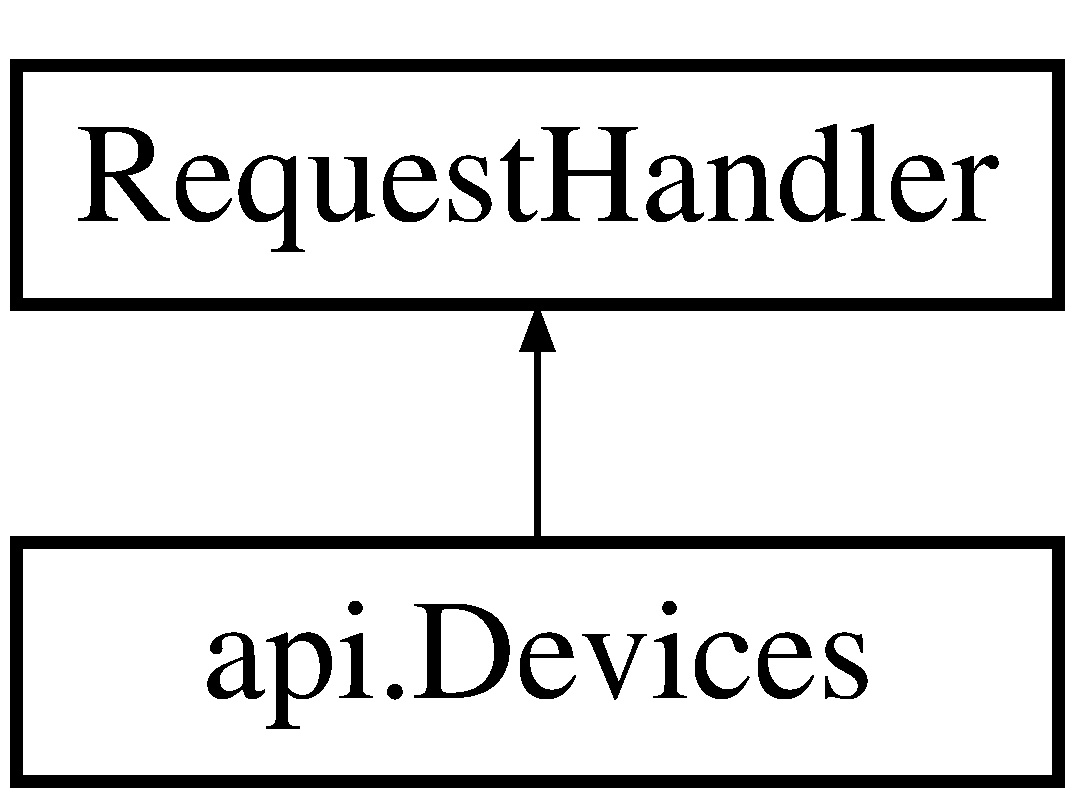
\includegraphics[height=2.000000cm]{classapi_1_1_devices}
\end{center}
\end{figure}
\subsection*{Public Member Functions}
\begin{DoxyCompactItemize}
\item 
def \hyperlink{classapi_1_1_devices_a695093fde641d0b21cecfca0c3c9d4c0}{get}
\item 
def \hyperlink{classapi_1_1_devices_accb6dbcf0fa656cfbab95553867ece1b}{post}
\end{DoxyCompactItemize}


\subsection{Member Function Documentation}
\hypertarget{classapi_1_1_devices_a695093fde641d0b21cecfca0c3c9d4c0}{\index{api\-::\-Devices@{api\-::\-Devices}!get@{get}}
\index{get@{get}!api::Devices@{api\-::\-Devices}}
\subsubsection[{get}]{\setlength{\rightskip}{0pt plus 5cm}def api.\-Devices.\-get (
\begin{DoxyParamCaption}
\item[{}]{self}
\end{DoxyParamCaption}
)}}\label{classapi_1_1_devices_a695093fde641d0b21cecfca0c3c9d4c0}
\begin{DoxyVerb}GET: returns the Devices registered.\end{DoxyVerb}
 \hypertarget{classapi_1_1_devices_accb6dbcf0fa656cfbab95553867ece1b}{\index{api\-::\-Devices@{api\-::\-Devices}!post@{post}}
\index{post@{post}!api::Devices@{api\-::\-Devices}}
\subsubsection[{post}]{\setlength{\rightskip}{0pt plus 5cm}def api.\-Devices.\-post (
\begin{DoxyParamCaption}
\item[{}]{self}
\end{DoxyParamCaption}
)}}\label{classapi_1_1_devices_accb6dbcf0fa656cfbab95553867ece1b}
\begin{DoxyVerb}POST: adds a new Device.

Post data must contain valid Device object.
\end{DoxyVerb}
 

The documentation for this class was generated from the following file\-:\begin{DoxyCompactItemize}
\item 
api.\-py\end{DoxyCompactItemize}

\hypertarget{classhailingfrequency_1_1_hailing_frequency}{\section{hailingfrequency.\-Hailing\-Frequency Class Reference}
\label{classhailingfrequency_1_1_hailing_frequency}\index{hailingfrequency.\-Hailing\-Frequency@{hailingfrequency.\-Hailing\-Frequency}}
}
Inheritance diagram for hailingfrequency.\-Hailing\-Frequency\-:\begin{figure}[H]
\begin{center}
\leavevmode
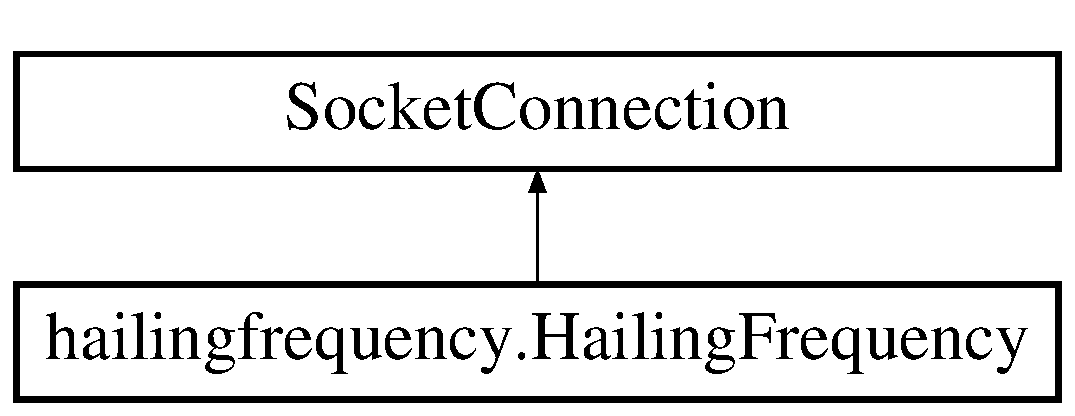
\includegraphics[height=2.000000cm]{classhailingfrequency_1_1_hailing_frequency}
\end{center}
\end{figure}
\subsection*{Public Member Functions}
\begin{DoxyCompactItemize}
\item 
\hypertarget{classhailingfrequency_1_1_hailing_frequency_a43ef95e6ea485f5d6f3237cffcffc2e8}{def {\bfseries on\-\_\-open}}\label{classhailingfrequency_1_1_hailing_frequency_a43ef95e6ea485f5d6f3237cffcffc2e8}

\item 
\hypertarget{classhailingfrequency_1_1_hailing_frequency_a6cd98bd788ac92a75717ea4eebc7ece5}{def {\bfseries on\-\_\-message}}\label{classhailingfrequency_1_1_hailing_frequency_a6cd98bd788ac92a75717ea4eebc7ece5}

\item 
\hypertarget{classhailingfrequency_1_1_hailing_frequency_a2b4502d47401f769da2d025af35df25e}{def {\bfseries on\-\_\-close}}\label{classhailingfrequency_1_1_hailing_frequency_a2b4502d47401f769da2d025af35df25e}

\end{DoxyCompactItemize}
\subsection*{Static Public Attributes}
\begin{DoxyCompactItemize}
\item 
\hypertarget{classhailingfrequency_1_1_hailing_frequency_a0e09ad983a40863402e49ed9e69e463d}{tuple {\bfseries participants} = set()}\label{classhailingfrequency_1_1_hailing_frequency_a0e09ad983a40863402e49ed9e69e463d}

\end{DoxyCompactItemize}


The documentation for this class was generated from the following file\-:\begin{DoxyCompactItemize}
\item 
hailingfrequency.\-py\end{DoxyCompactItemize}

\hypertarget{classhailingfrequency_1_1_hailing_frequency_handler}{\section{hailingfrequency.\-Hailing\-Frequency\-Handler Class Reference}
\label{classhailingfrequency_1_1_hailing_frequency_handler}\index{hailingfrequency.\-Hailing\-Frequency\-Handler@{hailingfrequency.\-Hailing\-Frequency\-Handler}}
}
Inheritance diagram for hailingfrequency.\-Hailing\-Frequency\-Handler\-:\begin{figure}[H]
\begin{center}
\leavevmode
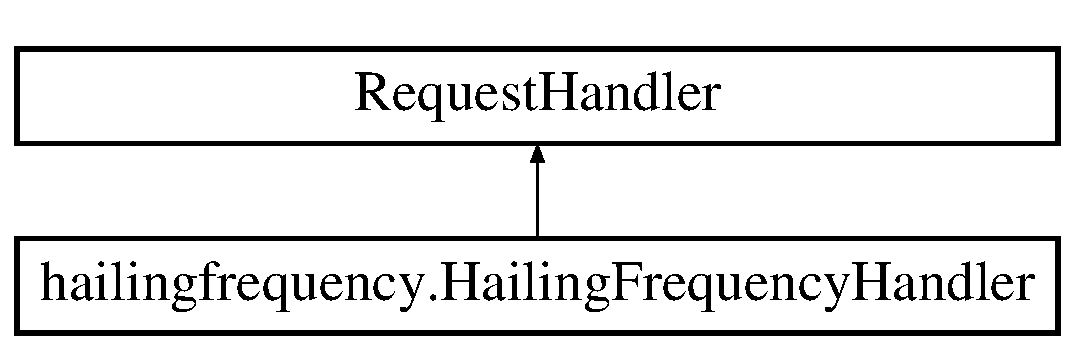
\includegraphics[height=2.000000cm]{classhailingfrequency_1_1_hailing_frequency_handler}
\end{center}
\end{figure}
\subsection*{Public Member Functions}
\begin{DoxyCompactItemize}
\item 
\hypertarget{classhailingfrequency_1_1_hailing_frequency_handler_a0bda90585d0261bea07e6db3077d6f79}{def {\bfseries get}}\label{classhailingfrequency_1_1_hailing_frequency_handler_a0bda90585d0261bea07e6db3077d6f79}

\end{DoxyCompactItemize}


The documentation for this class was generated from the following file\-:\begin{DoxyCompactItemize}
\item 
hailingfrequency.\-py\end{DoxyCompactItemize}

\hypertarget{classapi_1_1_nest}{\section{api.\-Nest Class Reference}
\label{classapi_1_1_nest}\index{api.\-Nest@{api.\-Nest}}
}
Inheritance diagram for api.\-Nest\-:\begin{figure}[H]
\begin{center}
\leavevmode
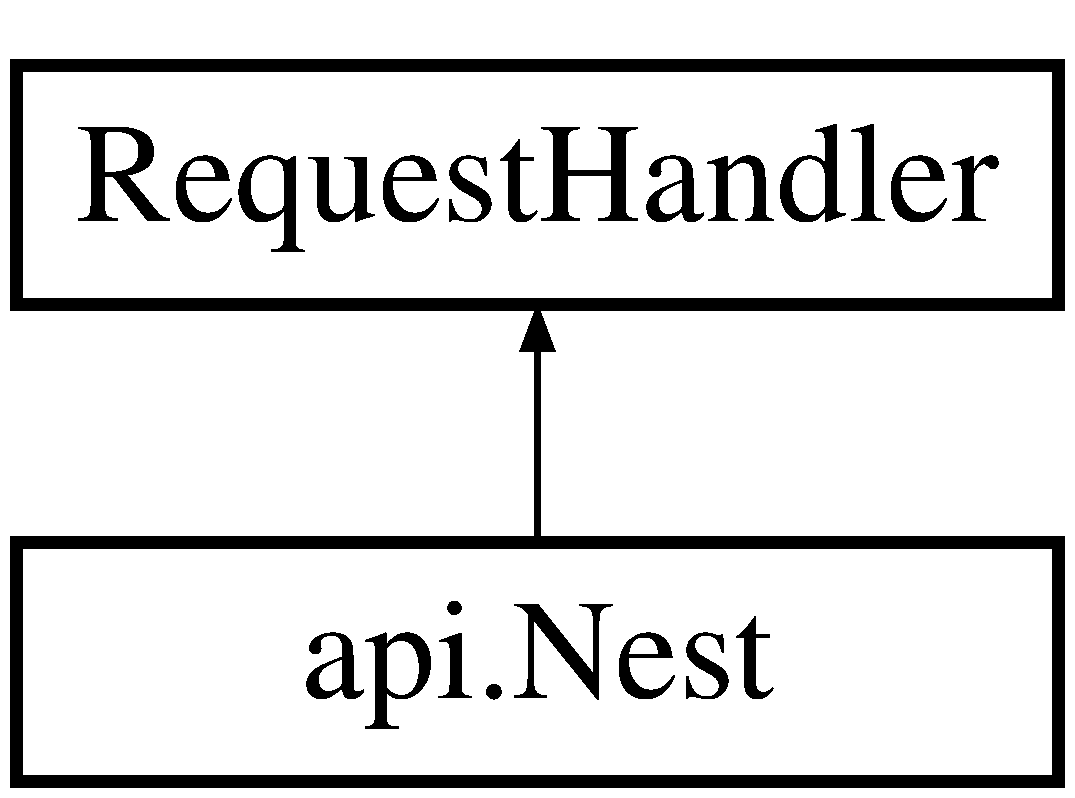
\includegraphics[height=2.000000cm]{classapi_1_1_nest}
\end{center}
\end{figure}
\subsection*{Public Member Functions}
\begin{DoxyCompactItemize}
\item 
\hypertarget{classapi_1_1_nest_ac63c05297a0c2a9ef7c4d78649bd6882}{def {\bfseries initialize}}\label{classapi_1_1_nest_ac63c05297a0c2a9ef7c4d78649bd6882}

\item 
def \hyperlink{classapi_1_1_nest_abc52411100635182cbd712b9f3014ea8}{get}
\item 
def \hyperlink{classapi_1_1_nest_a1b722ddb518afce74b5a59be42e7af09}{put}
\item 
def \hyperlink{classapi_1_1_nest_a224057785cc58de52b2fb5ba9edbb044}{delete}
\end{DoxyCompactItemize}
\subsection*{Public Attributes}
\begin{DoxyCompactItemize}
\item 
\hypertarget{classapi_1_1_nest_a4aae8cb29281cfd74c4c975fe309d612}{{\bfseries nest\-Id}}\label{classapi_1_1_nest_a4aae8cb29281cfd74c4c975fe309d612}

\end{DoxyCompactItemize}


\subsection{Member Function Documentation}
\hypertarget{classapi_1_1_nest_a224057785cc58de52b2fb5ba9edbb044}{\index{api\-::\-Nest@{api\-::\-Nest}!delete@{delete}}
\index{delete@{delete}!api::Nest@{api\-::\-Nest}}
\subsubsection[{delete}]{\setlength{\rightskip}{0pt plus 5cm}def api.\-Nest.\-delete (
\begin{DoxyParamCaption}
\item[{}]{self, }
\item[{}]{nest\-Id}
\end{DoxyParamCaption}
)}}\label{classapi_1_1_nest_a224057785cc58de52b2fb5ba9edbb044}
\begin{DoxyVerb}DELETE: deletes the Nest.\end{DoxyVerb}
 \hypertarget{classapi_1_1_nest_abc52411100635182cbd712b9f3014ea8}{\index{api\-::\-Nest@{api\-::\-Nest}!get@{get}}
\index{get@{get}!api::Nest@{api\-::\-Nest}}
\subsubsection[{get}]{\setlength{\rightskip}{0pt plus 5cm}def api.\-Nest.\-get (
\begin{DoxyParamCaption}
\item[{}]{self, }
\item[{}]{nest\-Id}
\end{DoxyParamCaption}
)}}\label{classapi_1_1_nest_abc52411100635182cbd712b9f3014ea8}
\begin{DoxyVerb}GET: returns the Nest matching specified id.\end{DoxyVerb}
 \hypertarget{classapi_1_1_nest_a1b722ddb518afce74b5a59be42e7af09}{\index{api\-::\-Nest@{api\-::\-Nest}!put@{put}}
\index{put@{put}!api::Nest@{api\-::\-Nest}}
\subsubsection[{put}]{\setlength{\rightskip}{0pt plus 5cm}def api.\-Nest.\-put (
\begin{DoxyParamCaption}
\item[{}]{self, }
\item[{}]{user\-Id}
\end{DoxyParamCaption}
)}}\label{classapi_1_1_nest_a1b722ddb518afce74b5a59be42e7af09}
\begin{DoxyVerb}PUT: updates the Nest's data.\end{DoxyVerb}
 

The documentation for this class was generated from the following file\-:\begin{DoxyCompactItemize}
\item 
api.\-py\end{DoxyCompactItemize}

\hypertarget{classnest_1_1_nest}{\section{nest.\-Nest Class Reference}
\label{classnest_1_1_nest}\index{nest.\-Nest@{nest.\-Nest}}
}
Inheritance diagram for nest.\-Nest\-:\begin{figure}[H]
\begin{center}
\leavevmode
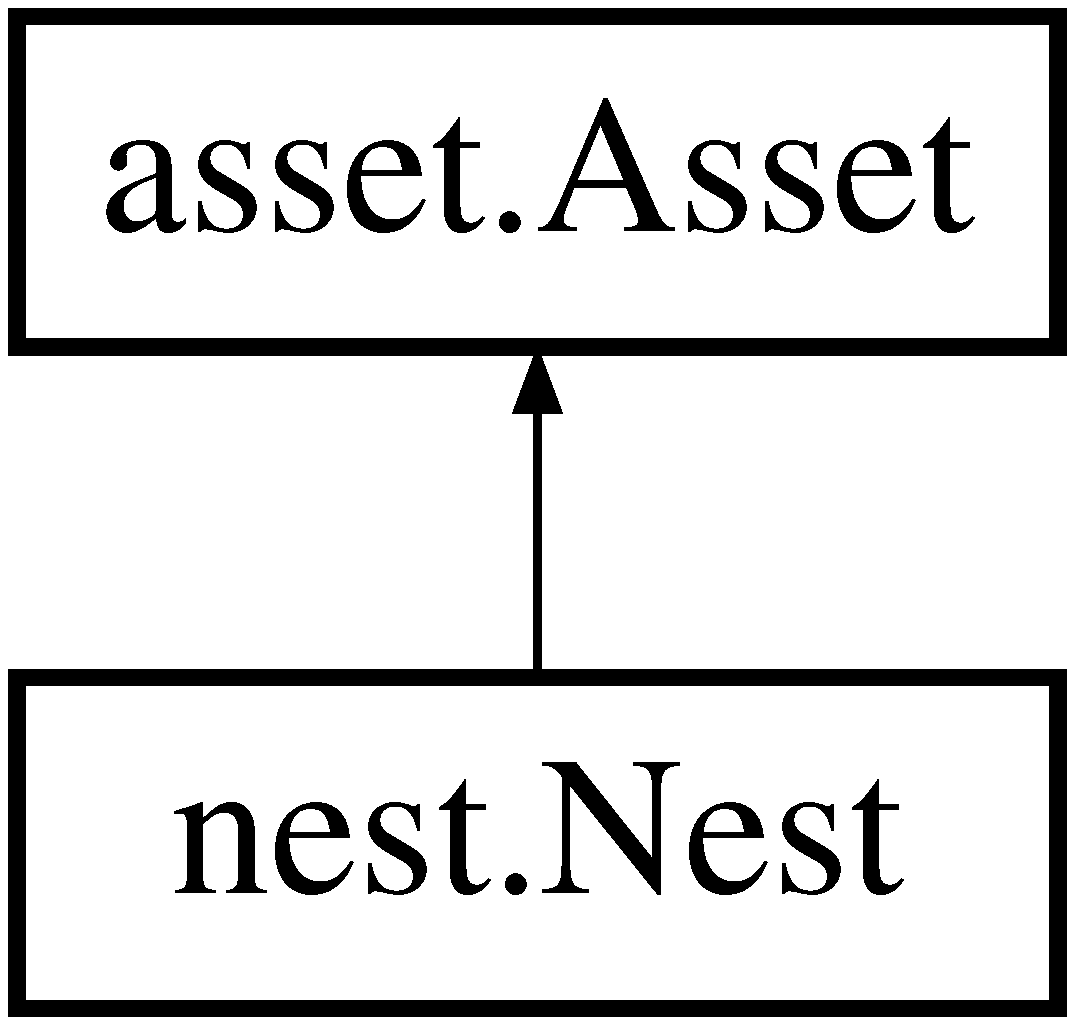
\includegraphics[height=2.000000cm]{classnest_1_1_nest}
\end{center}
\end{figure}
\subsection*{Public Member Functions}
\begin{DoxyCompactItemize}
\item 
\hypertarget{classnest_1_1_nest_a6ea507631915e9b1e54c1e091e19d63f}{def {\bfseries \-\_\-\-\_\-init\-\_\-\-\_\-}}\label{classnest_1_1_nest_a6ea507631915e9b1e54c1e091e19d63f}

\item 
def \hyperlink{classnest_1_1_nest_a3e9ae5e34ea2f5fe44d9a8f2e42822dc}{create}
\end{DoxyCompactItemize}
\subsection*{Public Attributes}
\begin{DoxyCompactItemize}
\item 
\hypertarget{classnest_1_1_nest_aa2a7d17fd5260f5b6bf96ead594b7029}{{\bfseries members}}\label{classnest_1_1_nest_aa2a7d17fd5260f5b6bf96ead594b7029}

\item 
\hypertarget{classnest_1_1_nest_a6ff95598ec58152e955ef1230fede31e}{{\bfseries devices}}\label{classnest_1_1_nest_a6ff95598ec58152e955ef1230fede31e}

\end{DoxyCompactItemize}
\subsection*{Additional Inherited Members}


\subsection{Member Function Documentation}
\hypertarget{classnest_1_1_nest_a3e9ae5e34ea2f5fe44d9a8f2e42822dc}{\index{nest\-::\-Nest@{nest\-::\-Nest}!create@{create}}
\index{create@{create}!nest::Nest@{nest\-::\-Nest}}
\subsubsection[{create}]{\setlength{\rightskip}{0pt plus 5cm}def nest.\-Nest.\-create (
\begin{DoxyParamCaption}
\item[{}]{self}
\end{DoxyParamCaption}
)}}\label{classnest_1_1_nest_a3e9ae5e34ea2f5fe44d9a8f2e42822dc}
\begin{DoxyVerb}Creates a new Nest, and sets its id.\end{DoxyVerb}
 

The documentation for this class was generated from the following file\-:\begin{DoxyCompactItemize}
\item 
nest.\-py\end{DoxyCompactItemize}

\hypertarget{classapi_1_1_nests}{\section{api.\-Nests Class Reference}
\label{classapi_1_1_nests}\index{api.\-Nests@{api.\-Nests}}
}
Inheritance diagram for api.\-Nests\-:\begin{figure}[H]
\begin{center}
\leavevmode
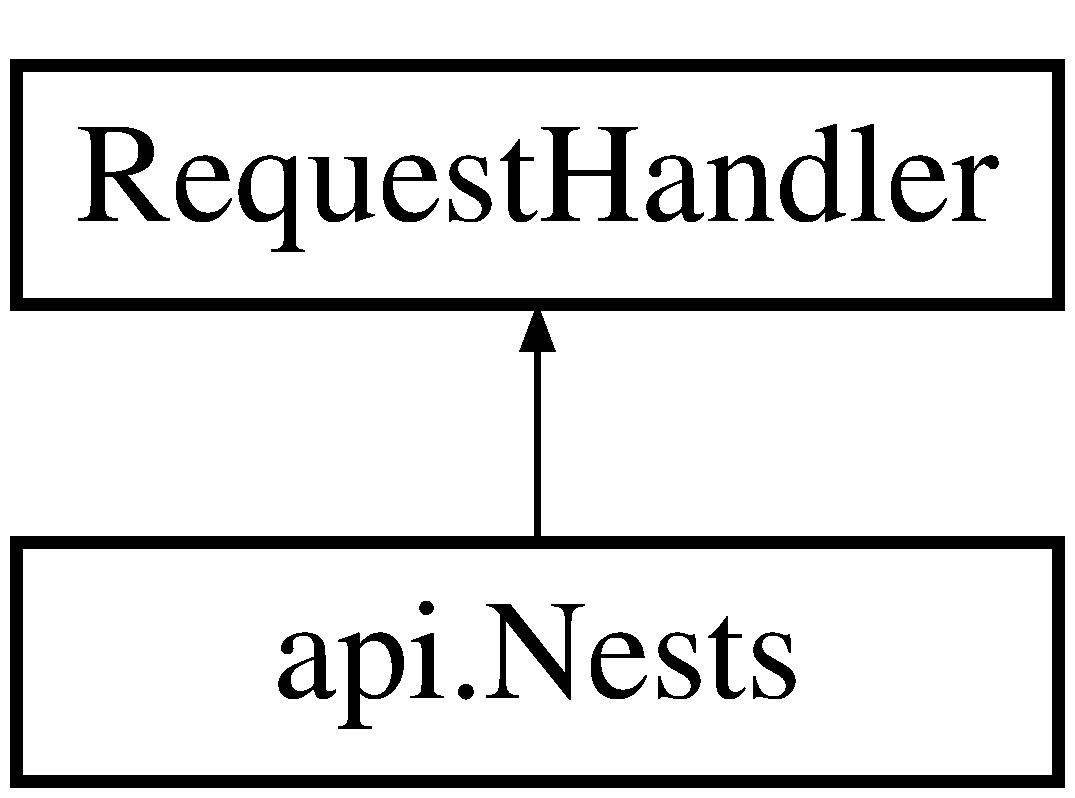
\includegraphics[height=2.000000cm]{classapi_1_1_nests}
\end{center}
\end{figure}
\subsection*{Public Member Functions}
\begin{DoxyCompactItemize}
\item 
def \hyperlink{classapi_1_1_nests_aee226cdcaacc8be98e80f1b27626f9ec}{get}
\item 
def \hyperlink{classapi_1_1_nests_aa0894a39e2ff51986c333fd19ef2cd34}{post}
\end{DoxyCompactItemize}


\subsection{Member Function Documentation}
\hypertarget{classapi_1_1_nests_aee226cdcaacc8be98e80f1b27626f9ec}{\index{api\-::\-Nests@{api\-::\-Nests}!get@{get}}
\index{get@{get}!api::Nests@{api\-::\-Nests}}
\subsubsection[{get}]{\setlength{\rightskip}{0pt plus 5cm}def api.\-Nests.\-get (
\begin{DoxyParamCaption}
\item[{}]{self}
\end{DoxyParamCaption}
)}}\label{classapi_1_1_nests_aee226cdcaacc8be98e80f1b27626f9ec}
\begin{DoxyVerb}GET: returns the Nests registered.\end{DoxyVerb}
 \hypertarget{classapi_1_1_nests_aa0894a39e2ff51986c333fd19ef2cd34}{\index{api\-::\-Nests@{api\-::\-Nests}!post@{post}}
\index{post@{post}!api::Nests@{api\-::\-Nests}}
\subsubsection[{post}]{\setlength{\rightskip}{0pt plus 5cm}def api.\-Nests.\-post (
\begin{DoxyParamCaption}
\item[{}]{self}
\end{DoxyParamCaption}
)}}\label{classapi_1_1_nests_aa0894a39e2ff51986c333fd19ef2cd34}
\begin{DoxyVerb}POST: adds a new Nest.

Post data must contain valid Nest object.
\end{DoxyVerb}
 

The documentation for this class was generated from the following file\-:\begin{DoxyCompactItemize}
\item 
api.\-py\end{DoxyCompactItemize}

\hypertarget{classapi_1_1_ping}{\section{api.\-Ping Class Reference}
\label{classapi_1_1_ping}\index{api.\-Ping@{api.\-Ping}}
}
Inheritance diagram for api.\-Ping\-:\begin{figure}[H]
\begin{center}
\leavevmode
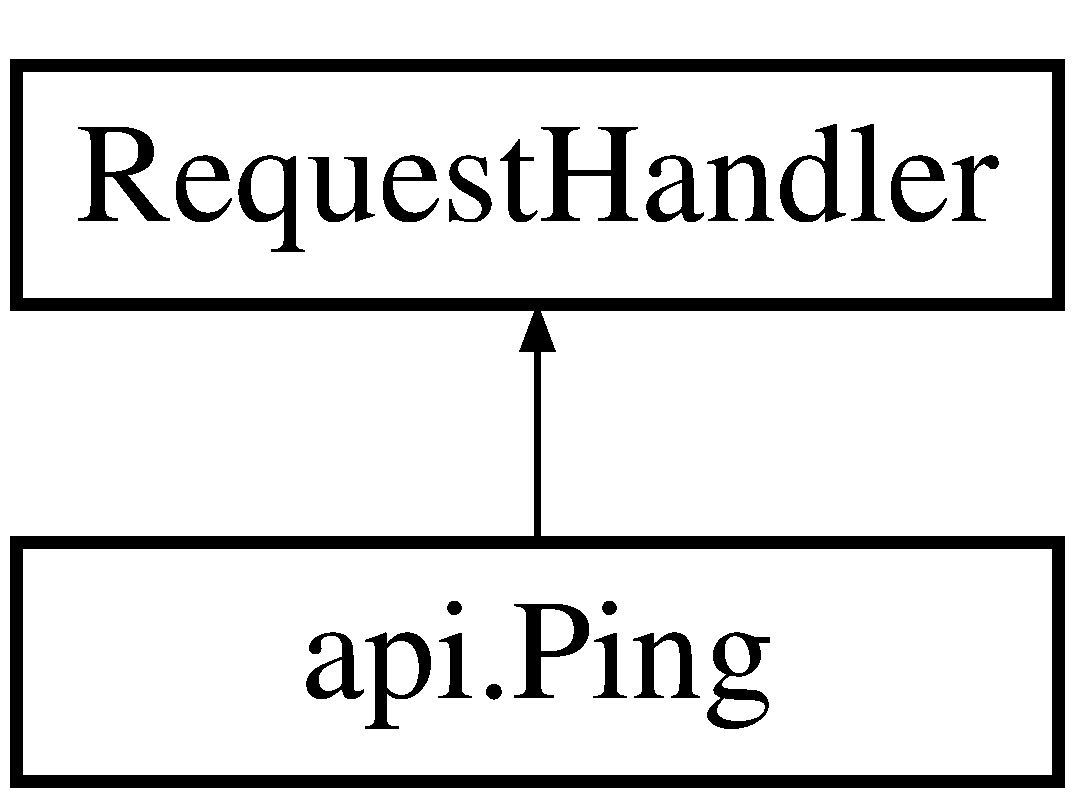
\includegraphics[height=2.000000cm]{classapi_1_1_ping}
\end{center}
\end{figure}
\subsection*{Public Member Functions}
\begin{DoxyCompactItemize}
\item 
\hypertarget{classapi_1_1_ping_a45732451f2e292e44dd204127920255d}{def {\bfseries initialize}}\label{classapi_1_1_ping_a45732451f2e292e44dd204127920255d}

\item 
def \hyperlink{classapi_1_1_ping_a6082e3e7608059cd50e92b116eaee580}{post}
\end{DoxyCompactItemize}
\subsection*{Public Attributes}
\begin{DoxyCompactItemize}
\item 
\hypertarget{classapi_1_1_ping_affa752457ec1a022bffd77fb58afc2b3}{{\bfseries entity\-Id}}\label{classapi_1_1_ping_affa752457ec1a022bffd77fb58afc2b3}

\item 
\hypertarget{classapi_1_1_ping_ae4e0ce63a966a74226524f07385b2cbe}{{\bfseries action}}\label{classapi_1_1_ping_ae4e0ce63a966a74226524f07385b2cbe}

\end{DoxyCompactItemize}


\subsection{Member Function Documentation}
\hypertarget{classapi_1_1_ping_a6082e3e7608059cd50e92b116eaee580}{\index{api\-::\-Ping@{api\-::\-Ping}!post@{post}}
\index{post@{post}!api::Ping@{api\-::\-Ping}}
\subsubsection[{post}]{\setlength{\rightskip}{0pt plus 5cm}def api.\-Ping.\-post (
\begin{DoxyParamCaption}
\item[{}]{self, }
\item[{}]{entity\-Id, }
\item[{}]{action\-Id}
\end{DoxyParamCaption}
)}}\label{classapi_1_1_ping_a6082e3e7608059cd50e92b116eaee580}
\begin{DoxyVerb}POST: sends a ping (event notification) to the specified entity, with action specified by the Action argument\end{DoxyVerb}
 

The documentation for this class was generated from the following file\-:\begin{DoxyCompactItemize}
\item 
api.\-py\end{DoxyCompactItemize}

\hypertarget{classhailingfrequency_1_1_router}{\section{hailingfrequency.\-Router Class Reference}
\label{classhailingfrequency_1_1_router}\index{hailingfrequency.\-Router@{hailingfrequency.\-Router}}
}
Inheritance diagram for hailingfrequency.\-Router\-:\begin{figure}[H]
\begin{center}
\leavevmode
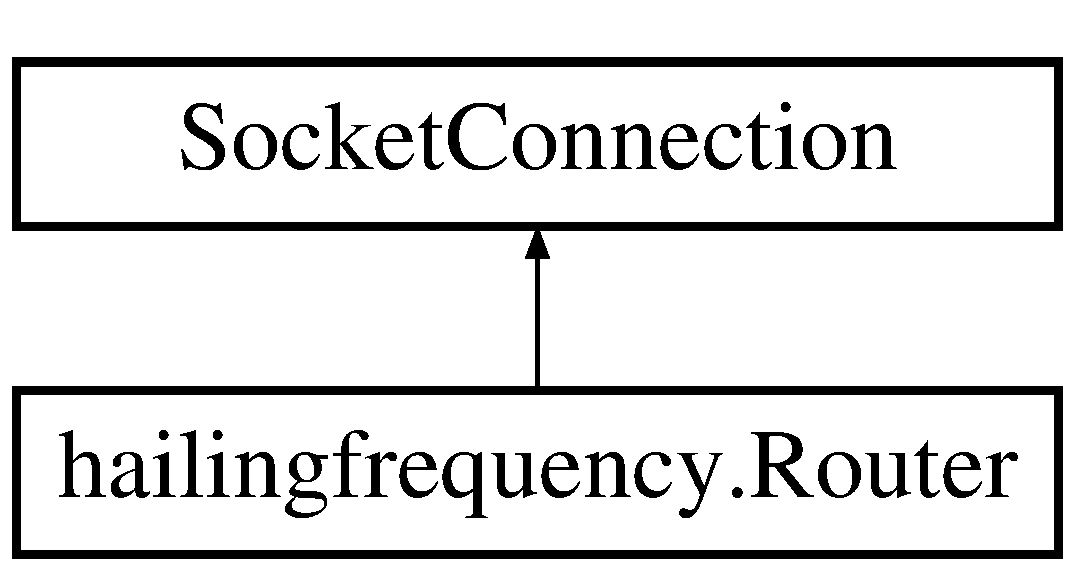
\includegraphics[height=2.000000cm]{classhailingfrequency_1_1_router}
\end{center}
\end{figure}
\subsection*{Static Public Attributes}
\begin{DoxyCompactItemize}
\item 
\hypertarget{classhailingfrequency_1_1_router_abd092ba4b038043ee08bc33112758c7a}{list {\bfseries ep} = \mbox{[}'/herpie','/derpie','/derpderp'\mbox{]}}\label{classhailingfrequency_1_1_router_abd092ba4b038043ee08bc33112758c7a}

\end{DoxyCompactItemize}


The documentation for this class was generated from the following file\-:\begin{DoxyCompactItemize}
\item 
hailingfrequency.\-py\end{DoxyCompactItemize}

\hypertarget{classhailingfrequency_1_1_socket_i_o_handler}{\section{hailingfrequency.\-Socket\-I\-O\-Handler Class Reference}
\label{classhailingfrequency_1_1_socket_i_o_handler}\index{hailingfrequency.\-Socket\-I\-O\-Handler@{hailingfrequency.\-Socket\-I\-O\-Handler}}
}
Inheritance diagram for hailingfrequency.\-Socket\-I\-O\-Handler\-:\begin{figure}[H]
\begin{center}
\leavevmode
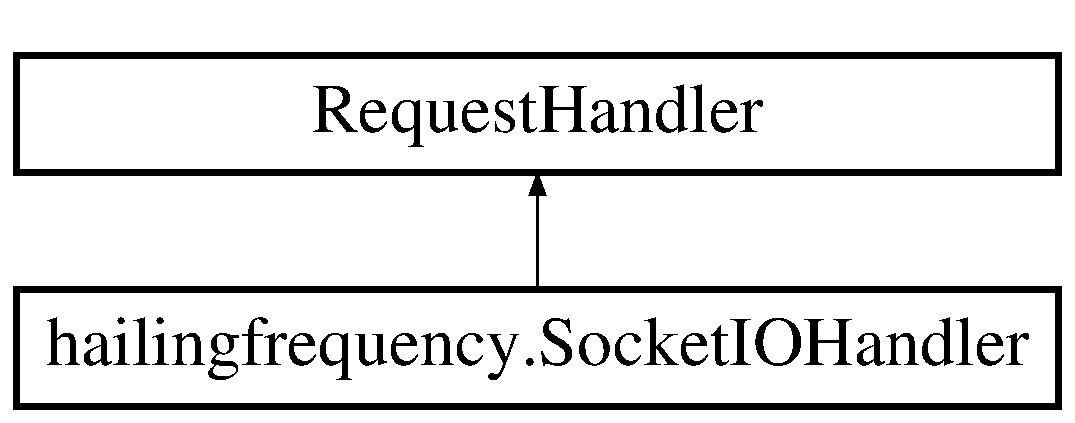
\includegraphics[height=2.000000cm]{classhailingfrequency_1_1_socket_i_o_handler}
\end{center}
\end{figure}
\subsection*{Public Member Functions}
\begin{DoxyCompactItemize}
\item 
\hypertarget{classhailingfrequency_1_1_socket_i_o_handler_a344624a70ebaa23998ce598a0dedbdc7}{def {\bfseries get}}\label{classhailingfrequency_1_1_socket_i_o_handler_a344624a70ebaa23998ce598a0dedbdc7}

\end{DoxyCompactItemize}


The documentation for this class was generated from the following file\-:\begin{DoxyCompactItemize}
\item 
hailingfrequency.\-py\end{DoxyCompactItemize}

\hypertarget{classuser_1_1_user}{\section{user.\-User Class Reference}
\label{classuser_1_1_user}\index{user.\-User@{user.\-User}}
}
Inheritance diagram for user.\-User\-:\begin{figure}[H]
\begin{center}
\leavevmode
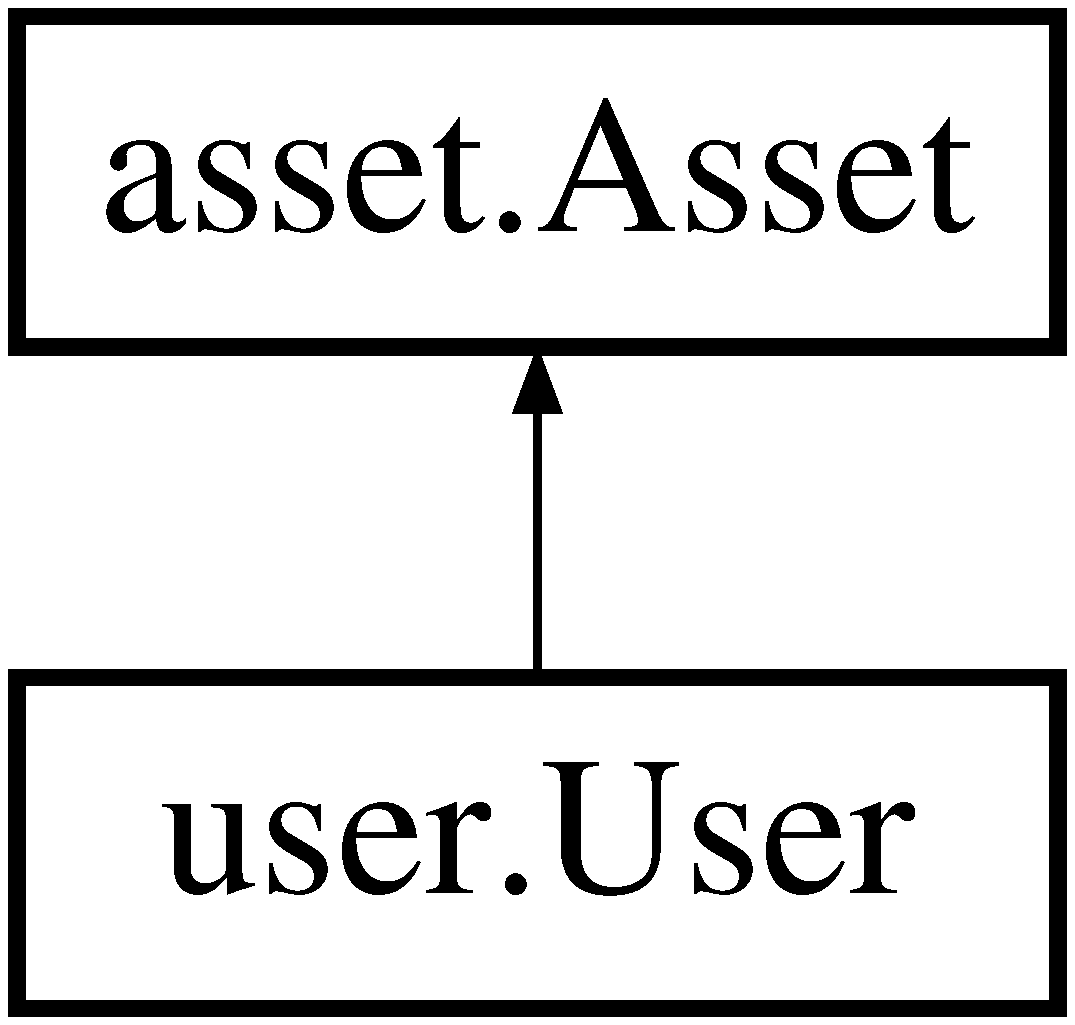
\includegraphics[height=2.000000cm]{classuser_1_1_user}
\end{center}
\end{figure}
\subsection*{Public Member Functions}
\begin{DoxyCompactItemize}
\item 
\hypertarget{classuser_1_1_user_af37c1e601519fef697f986c3334e0bf0}{def {\bfseries \-\_\-\-\_\-init\-\_\-\-\_\-}}\label{classuser_1_1_user_af37c1e601519fef697f986c3334e0bf0}

\item 
def \hyperlink{classuser_1_1_user_a537f4e3e8b43f40882b9b149e7adca2e}{create}
\item 
def \hyperlink{classuser_1_1_user_a05d0ea577c0ad94aa421dc9628de1de3}{add\-To\-Nest}
\item 
def \hyperlink{classuser_1_1_user_a05d0ea577c0ad94aa421dc9628de1de3}{add\-To\-Nest}
\end{DoxyCompactItemize}
\subsection*{Public Attributes}
\begin{DoxyCompactItemize}
\item 
\hypertarget{classuser_1_1_user_ac6ba5d5b3449c476080ddcf1397ac104}{{\bfseries nests}}\label{classuser_1_1_user_ac6ba5d5b3449c476080ddcf1397ac104}

\end{DoxyCompactItemize}
\subsection*{Additional Inherited Members}


\subsection{Detailed Description}
\begin{DoxyVerb}The User class\end{DoxyVerb}
 

\subsection{Member Function Documentation}
\hypertarget{classuser_1_1_user_a05d0ea577c0ad94aa421dc9628de1de3}{\index{user\-::\-User@{user\-::\-User}!add\-To\-Nest@{add\-To\-Nest}}
\index{add\-To\-Nest@{add\-To\-Nest}!user::User@{user\-::\-User}}
\subsubsection[{add\-To\-Nest}]{\setlength{\rightskip}{0pt plus 5cm}def user.\-User.\-add\-To\-Nest (
\begin{DoxyParamCaption}
\item[{}]{self, }
\item[{}]{nest\-Id = {\ttfamily None}}
\end{DoxyParamCaption}
)}}\label{classuser_1_1_user_a05d0ea577c0ad94aa421dc9628de1de3}
\begin{DoxyVerb}Adds User to a Nest\end{DoxyVerb}
 \hypertarget{classuser_1_1_user_a05d0ea577c0ad94aa421dc9628de1de3}{\index{user\-::\-User@{user\-::\-User}!add\-To\-Nest@{add\-To\-Nest}}
\index{add\-To\-Nest@{add\-To\-Nest}!user::User@{user\-::\-User}}
\subsubsection[{add\-To\-Nest}]{\setlength{\rightskip}{0pt plus 5cm}def user.\-User.\-add\-To\-Nest (
\begin{DoxyParamCaption}
\item[{}]{self, }
\item[{}]{nest\-Id = {\ttfamily None}}
\end{DoxyParamCaption}
)}}\label{classuser_1_1_user_a05d0ea577c0ad94aa421dc9628de1de3}
\begin{DoxyVerb}Adds User to a Nest\end{DoxyVerb}
 \hypertarget{classuser_1_1_user_a537f4e3e8b43f40882b9b149e7adca2e}{\index{user\-::\-User@{user\-::\-User}!create@{create}}
\index{create@{create}!user::User@{user\-::\-User}}
\subsubsection[{create}]{\setlength{\rightskip}{0pt plus 5cm}def user.\-User.\-create (
\begin{DoxyParamCaption}
\item[{}]{self}
\end{DoxyParamCaption}
)}}\label{classuser_1_1_user_a537f4e3e8b43f40882b9b149e7adca2e}
\begin{DoxyVerb}Creates a new User, and sets its id.\end{DoxyVerb}
 

The documentation for this class was generated from the following file\-:\begin{DoxyCompactItemize}
\item 
user.\-py\end{DoxyCompactItemize}

\hypertarget{classapi_1_1_user}{\section{api.\-User Class Reference}
\label{classapi_1_1_user}\index{api.\-User@{api.\-User}}
}
Inheritance diagram for api.\-User\-:\begin{figure}[H]
\begin{center}
\leavevmode
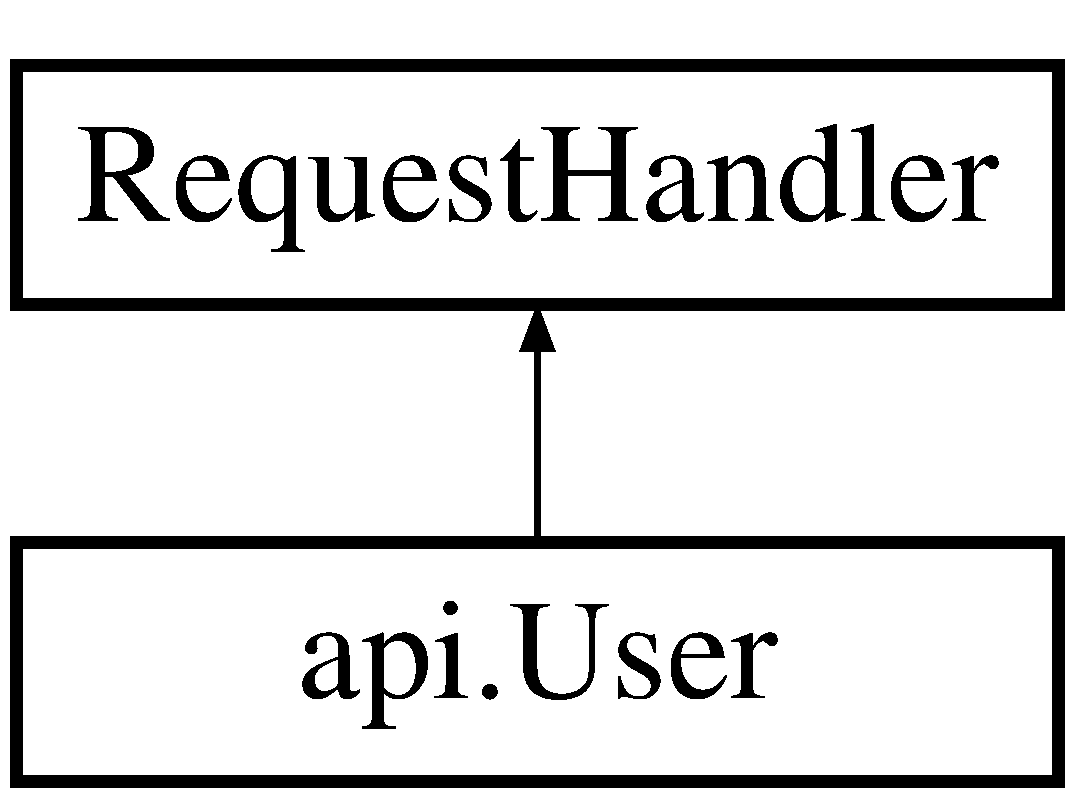
\includegraphics[height=2.000000cm]{classapi_1_1_user}
\end{center}
\end{figure}
\subsection*{Public Member Functions}
\begin{DoxyCompactItemize}
\item 
\hypertarget{classapi_1_1_user_a0f2cf0a3d4c5d606953358cb92a2b166}{def {\bfseries initialize}}\label{classapi_1_1_user_a0f2cf0a3d4c5d606953358cb92a2b166}

\item 
def \hyperlink{classapi_1_1_user_afd5bb645380fe6192ec6068fdcdda96e}{get}
\item 
def \hyperlink{classapi_1_1_user_a9365de26fbc9d590fce399ddf775a28f}{post}
\item 
def \hyperlink{classapi_1_1_user_aefffd1aa5d149b091f779b3222748fb5}{put}
\item 
def \hyperlink{classapi_1_1_user_a2868600f2d73a2e59e4a814205e5ae6e}{delete}
\end{DoxyCompactItemize}
\subsection*{Public Attributes}
\begin{DoxyCompactItemize}
\item 
\hypertarget{classapi_1_1_user_ad10ba6df28dbfe8546f24226c1ca28f6}{{\bfseries user\-Id}}\label{classapi_1_1_user_ad10ba6df28dbfe8546f24226c1ca28f6}

\end{DoxyCompactItemize}


\subsection{Member Function Documentation}
\hypertarget{classapi_1_1_user_a2868600f2d73a2e59e4a814205e5ae6e}{\index{api\-::\-User@{api\-::\-User}!delete@{delete}}
\index{delete@{delete}!api::User@{api\-::\-User}}
\subsubsection[{delete}]{\setlength{\rightskip}{0pt plus 5cm}def api.\-User.\-delete (
\begin{DoxyParamCaption}
\item[{}]{self, }
\item[{}]{nest\-Id}
\end{DoxyParamCaption}
)}}\label{classapi_1_1_user_a2868600f2d73a2e59e4a814205e5ae6e}
\begin{DoxyVerb}DELETE: deletes the User.\end{DoxyVerb}
 \hypertarget{classapi_1_1_user_afd5bb645380fe6192ec6068fdcdda96e}{\index{api\-::\-User@{api\-::\-User}!get@{get}}
\index{get@{get}!api::User@{api\-::\-User}}
\subsubsection[{get}]{\setlength{\rightskip}{0pt plus 5cm}def api.\-User.\-get (
\begin{DoxyParamCaption}
\item[{}]{self, }
\item[{}]{user\-Id}
\end{DoxyParamCaption}
)}}\label{classapi_1_1_user_afd5bb645380fe6192ec6068fdcdda96e}
\begin{DoxyVerb}GET: returns the User matching specified id.\end{DoxyVerb}
 \hypertarget{classapi_1_1_user_a9365de26fbc9d590fce399ddf775a28f}{\index{api\-::\-User@{api\-::\-User}!post@{post}}
\index{post@{post}!api::User@{api\-::\-User}}
\subsubsection[{post}]{\setlength{\rightskip}{0pt plus 5cm}def api.\-User.\-post (
\begin{DoxyParamCaption}
\item[{}]{self, }
\item[{}]{user\-Id}
\end{DoxyParamCaption}
)}}\label{classapi_1_1_user_a9365de26fbc9d590fce399ddf775a28f}
\begin{DoxyVerb}POST: log in/out the User matching specified id.\end{DoxyVerb}
 \hypertarget{classapi_1_1_user_aefffd1aa5d149b091f779b3222748fb5}{\index{api\-::\-User@{api\-::\-User}!put@{put}}
\index{put@{put}!api::User@{api\-::\-User}}
\subsubsection[{put}]{\setlength{\rightskip}{0pt plus 5cm}def api.\-User.\-put (
\begin{DoxyParamCaption}
\item[{}]{self, }
\item[{}]{user\-Id}
\end{DoxyParamCaption}
)}}\label{classapi_1_1_user_aefffd1aa5d149b091f779b3222748fb5}
\begin{DoxyVerb}PUT: updates the User's data.\end{DoxyVerb}
 

The documentation for this class was generated from the following file\-:\begin{DoxyCompactItemize}
\item 
api.\-py\end{DoxyCompactItemize}

\hypertarget{classapi_1_1_users}{\section{api.\-Users Class Reference}
\label{classapi_1_1_users}\index{api.\-Users@{api.\-Users}}
}
Inheritance diagram for api.\-Users\-:\begin{figure}[H]
\begin{center}
\leavevmode
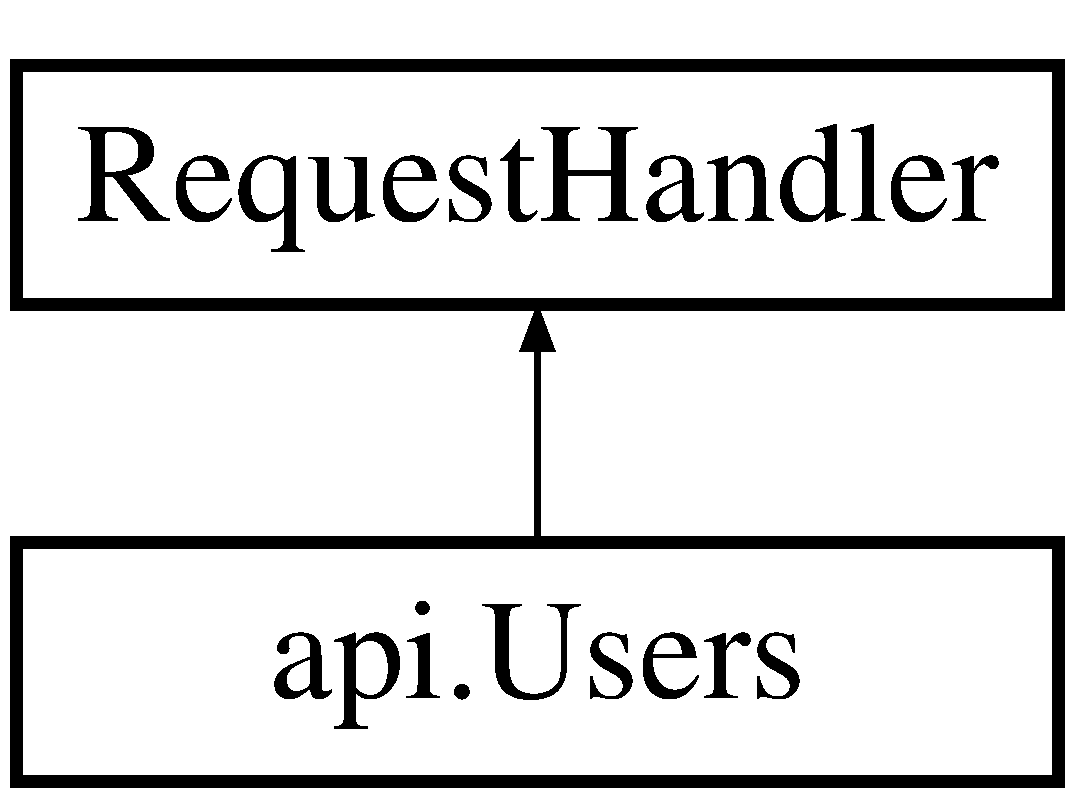
\includegraphics[height=2.000000cm]{classapi_1_1_users}
\end{center}
\end{figure}
\subsection*{Public Member Functions}
\begin{DoxyCompactItemize}
\item 
def \hyperlink{classapi_1_1_users_a5d177fece3eb6aa0e4bea1c5ddc07e36}{get}
\item 
def \hyperlink{classapi_1_1_users_a384872240d4628055a710f3082bfa356}{post}
\end{DoxyCompactItemize}


\subsection{Member Function Documentation}
\hypertarget{classapi_1_1_users_a5d177fece3eb6aa0e4bea1c5ddc07e36}{\index{api\-::\-Users@{api\-::\-Users}!get@{get}}
\index{get@{get}!api::Users@{api\-::\-Users}}
\subsubsection[{get}]{\setlength{\rightskip}{0pt plus 5cm}def api.\-Users.\-get (
\begin{DoxyParamCaption}
\item[{}]{self}
\end{DoxyParamCaption}
)}}\label{classapi_1_1_users_a5d177fece3eb6aa0e4bea1c5ddc07e36}
\begin{DoxyVerb}GET: returns a list of all Users [according to optional criteria].\end{DoxyVerb}
 \hypertarget{classapi_1_1_users_a384872240d4628055a710f3082bfa356}{\index{api\-::\-Users@{api\-::\-Users}!post@{post}}
\index{post@{post}!api::Users@{api\-::\-Users}}
\subsubsection[{post}]{\setlength{\rightskip}{0pt plus 5cm}def api.\-Users.\-post (
\begin{DoxyParamCaption}
\item[{}]{self}
\end{DoxyParamCaption}
)}}\label{classapi_1_1_users_a384872240d4628055a710f3082bfa356}
\begin{DoxyVerb}POST: creates a new User.

Post data must contain a valid User object.\end{DoxyVerb}
 

The documentation for this class was generated from the following file\-:\begin{DoxyCompactItemize}
\item 
api.\-py\end{DoxyCompactItemize}

%--- End generated contents ---

% Index
\newpage
\phantomsection
\addcontentsline{toc}{part}{Index}
\printindex

\end{document}
